%
%\documentclass[journal,peerreview]{IEEEtran}
\documentclass[journal,twoside]{IEEEtran}
%
% If IEEEtran.cls has not been installed into the LaTeX system files,
% manually specify the path to it like:
% \documentclass[journal]{../sty/IEEEtran}

\usepackage{cite}
% *** GRAPHICS RELATED PACKAGES ***
%
\usepackage[dvips]{graphicx}

%\renewcommand{\baselinestretch}{0.999}

% *** MATH PACKAGES ***
%
\usepackage[cmex10]{amsmath}
\interdisplaylinepenalty=2500
\usepackage{mathrsfs}
\usepackage{mathbbol}
\usepackage{amsbsy,amssymb}
\usepackage{alg}
\usepackage{array}
\usepackage[tight,footnotesize]{subfigure}
\usepackage{url}
\usepackage{psfrag}
\usepackage[usenames]{color}
\definecolor{DarkGreen}{rgb}{0,0.75,0.0}

\hyphenation{op-tical net-works semi-conduc-tor}

\def \TROTITLE {{ The Timid Night Watchman :\\ Controller Synthesis in the ``Real'' World}}
\def \SHORTTROTITLE {{ Controller Synthesis in the ``Real'' World }}

\newenvironment{definition}   
  {\begin{description}\setlength{\itemsep}{0pt}\setlength{\parsep}{0pt}
    \item[{\bf Definition:}]}
  {\end{description}}

% XXXX
\newenvironment{proof}   
  {\begin{description}\setlength{\itemsep}{0pt}\setlength{\parsep}{0pt}
    \item[{\bf Proof:}]}
    {\end{description}\begin{flushleft} $\Box$ \end{flushleft}}
\newtheorem{prop}{Proposition}
\newtheorem{lem}{Lemma}[section]
\newcommand{\reapp}[1]{Appendix~\ref{app:#1}}
\newcommand{\resec}[1]{Section~\ref{sec:#1}}
\newcommand{\req}[1]{(\ref{eqn:#1})}
\newcommand{\rechap}[1]{Chapter~\ref{chap:#1}}
\newcommand{\refig}[1]{Fig.~\ref{fig:#1}}
\newcommand{\retab}[1]{Table~\ref{tab:#1}}
\newcommand{\realg}[1]{Algorithm~\ref{alg:#1}}
\newcommand{\llem}[2]{\begin{lem}\label{lem:#1} #2 \end{lem}}
\newcommand{\relem}[1]{Lemma~\ref{lem:#1}}

\newcommand{ \prl } [1] {  \left( #1 \right) }
\newcommand{ \brl } [1] {  \left[ #1 \right] }
\newcommand{ \crl } [1] { \left\{ #1 \right\} }
\def \atan {\ensuremath{\mathrm{atan2}}}

\newcommand{\bbm}{\begin{bmatrix}}
\newcommand{\ebm}{\end{bmatrix}}
\newcommand{\mbf}{\mathbf}
\newcommand{ \mrm } [1] { \mathrm{ #1 } }
\newcommand{\bba}{\begin{array}}
\newcommand{\eba}{\end{array}}
\def \argmax {\operatornamewithlimits{arg\,max}}
\def \argmin {\operatornamewithlimits{arg\,min}}
\renewcommand{\lim} {\operatornamewithlimits{lim}}
\renewcommand{\min} {\operatornamewithlimits{min}}
\renewcommand{\max} {\operatornamewithlimits{max}}
\DeclareMathOperator*{\union} {\bigcup}
\newcommand{\ptwod}[2]{ \frac{\partial^2{#1}}{\partial{#2}^2 }  }
\newcommand{\pd}[2]{ \frac{\partial{#1}}{\partial{#2} }  }
\newcommand{\spec}[1] {\ensuremath{\left\lceil\!\!\left\rceil {#1}
                                         \right\lceil\!\!\right\rceil}}

\def \eg  {for example\ }
\def \ie  {\emph{i.e.\ }}
\newcommand{\absvl}[1]{ \left| #1 \right| }
\newcommand{\norm}[1]{ \left\| {#1} \right\| }
\def \ea  {\emph{et~al.}\ }
\def \R   {\ensuremath{\mrm{I\!R}}}
\def \r   {\R}
\def \Rn  {\ensuremath{\R^n}}
\def \Rt  {\ensuremath{\R^2}}
\def \B   {\ensuremath{\mathbf{\mathcal{B}}}} % Ball
\def \dB   {\ensuremath{\partial \B}} % Ball boundary
\def \dBi   {\ensuremath{\partial \B_{\mrm{in}}}} % Ball boundary
\def \dBe   {\ensuremath{\partial \B_{\mrm{out}}}} % Ball boundary
\def \vp  {\ensuremath{\varphi}}
\def \vpq {\ensuremath{\vp\!\prl{\pq}}}
\def \ra  {\ensuremath{\rightarrow}}
\def \pit {\ensuremath{\frac{\pi}{2}}}
\def \rt  {\ensuremath{\rl{2}}}
\def \pq  {\ensuremath{q}}
\def \qd  {\ensuremath{{q_d}}}
\def \qb  {\ensuremath{{q_b}}}
\def \qg  {\ensuremath{{q_\mrm{goal}}}}
\def \gg  {\ensuremath{{\gamma_\mrm{c}}}}
\def \Bmax {\ensuremath{\beta_{\mrm{max}}}}
\def \Bq   {\ensuremath{\beta\prl{\pq}}}
\def \Beta {\ensuremath{\beta}}
\def \qbmax {\ensuremath{\pq_\beta}}
\def \TR    {\ensuremath{T}}
\def \TRP  {\ensuremath{T\!\prl{\P}}}
\def \TRq  {\ensuremath{T\!\prl{\pq}}}
\def \zv  {\ensuremath{\mbf{0}}}
\def \gz {\ensuremath{{g_0}}}   % g vector
\def \X   {\ensuremath{X}}
\def \Xh  {\ensuremath{\hat{\X}}}
\def \Xoq {\ensuremath{\X\!\prl{\pq}}}
\def \Xhq {\ensuremath{\hat{\X}\!\prl{\pq}}}
\def \DtX {\ensuremath{\dot{\X}\!\prl{\pq}}} 
\def \dX  {\ensuremath{\dot{\X}}}
\def \DqX {\ensuremath{D_\pq \X}}
\def \DqXh {\ensuremath{D_\pq\Xh}}
\def \g  {\ensuremath{\gamma}}
\def \gd {\ensuremath{\gamma_d}}
\def \gb {\ensuremath{\gamma_b}}
\def \Dqg  {\ensuremath{D_\pq \gamma}}
\def \DqG  {\ensuremath{D_\pq \gamma}}
\def \DqbGb {\ensuremath{D_\qb \gamma_b}}
\def \DqGb {\ensuremath{D_{\varphi\!\prl{\pq}} \gamma_b}}
\def \DqP  {\ensuremath{D_\pq\varphi}}
\def \Soq  {\ensuremath{s\!\prl{\pq}}}
\def \DqGg {\ensuremath{D_\pq\!\gg}}
\def \Xhg  {\ensuremath{\hat{\X}_g}}
\def \Xgq  {\ensuremath{\X_g\!\prl{\pq}}}
\def \Sgq  {\ensuremath{s_g\!\prl{\pq}}}
\def \Mh   {\ensuremath{\hat{M}}}
\def \Nh   {\ensuremath{\hat{N}}}
\def \Ph   {\ensuremath{\hat{P}}}
\def \dqh  {\ensuremath{\dot{\hat{\pq}}}}
\def \Pv   {\ensuremath{P}}
\def \Qv   {\ensuremath{Q}}
\def \dQ   {\ensuremath{dQ}}
\def \u  {\ensuremath{u}}
\def \dq  {\ensuremath{\dot{\pq}}}
\def \ddq {\ensuremath{\ddot{\pq}}}
\def \Vmax {\ensuremath{\mathrm{V_{max}}}}
\def \Amax {\ensuremath{\mathrm{A_{max}}}}
\def \Umax {\ensuremath{\mathrm{A_{max}}}} % U max is max acceleration
\def \xv  {\ensuremath{\mbf{x}}}
\def \Ccomp {\ensuremath{\Phi_\P}}    % Component controller in cell \P
\def \Ccompt {\ensuremath{\Phi_{\P t}}}  % Component controller in cell \Pt

\def \CP     {\ensuremath{\Phi}}    % Generic control policy
\def \Cflow  {\ensuremath{\Phi_F}}  % Flow  control policy
\def \Calign {\ensuremath{\Phi_A}}  % Align control policy
\def \Csave  {\ensuremath{\Phi_S}}  % Save  control policy
\def \Cjoin  {\ensuremath{\Phi_J}} % Join  control policy
\def \Cgoal  {\ensuremath{\Phi_G}}  % Goal  control policy
\def \Ctrack {\ensuremath{\Phi_T}}  % Track control policy
\def \eh  {\ensuremath{\hat{e}}}
\def \vh  {\ensuremath{\hat{v}}}
\def \qh  {\ensuremath{\hat{\pq}}}
\def \dqh  {\ensuremath{\dot{\hat{\pq}}}}
\def \K   {\ensuremath{\mathcal{K}}} %  decomposition
\def \Vs  {\ensuremath{\mathcal{V}}} % Velocity limit set
\def \Us  {\ensuremath{\mathcal{U}}} %  collection of policies
\def \Usp  {\ensuremath{\Us^\prime}}
\def \Vs  {\ensuremath{\mathcal{V}}} % Velocity limit set
\def \As  {\ensuremath{\mathcal{A}}} % Acceleration limit set
\def \Zs  {\ensuremath{\mathcal{Z}}} % Aligned set
\def \Cs  {\ensuremath{\mathcal{C}}} % Collision free set
\def \Ss  {\ensuremath{\mathcal{S}}} % Saveable set
\def \L   {\ensuremath{\Lambda}}
\def \GL  {\ensuremath{\Gamma_{\Lambda}}} % prepares graph for \Us
\def \GpL {\ensuremath{\Gamma^\prime_{\Lambda}}} % partial order for \Us
\def \Lp  {\ensuremath{\Lambda^\prime}} %  ordered collection of policies
\newcommand{ \Do }[1]  {\ensuremath{\mathbf{\mathscr{D}}\!\prl{#1}}}
\newcommand{ \Go }[1]  {\ensuremath{\mathbf{\mathscr{G}}\!\prl{#1}}}
\def \pp  {\ensuremath{p}}
\def \nv  {\ensuremath{{n}}}
\def \ev  {\ensuremath{{e}}}

\newcommand{ \Ball }[2] {\ensuremath{\B\prl{{#1} , {#2} }}}
\newcommand{ \bigO }[1] {\ensuremath{\mbf{\mrm{O}}\prl{{#1}}}}

\def \P    {\ensuremath{\mathbf{\mathcal{P}}}} % Cell or Polytope
\def \Pt   {\ensuremath{\mathcal{P}_t}} % Target cell
\def \Ps   {\ensuremath{\mathcal{P}_s}} % Start cell
\def \Pg   {\ensuremath{\mathcal{P}_g}} % Goal cell
\def \Pi   {\ensuremath{\mathcal{P}_i}} % i^{th} cell
\def \Pj   {\ensuremath{\mathcal{P}_j}} % j^{th} cell
\def \D    {\ensuremath{\mathcal{D}}}   % Disk
\def \Pb   {\ensuremath{\bar{\mathbf{\mathcal{P}}}}} % Cell or Polytope
\def \vsurf {\ensuremath{\mathcal{V}}}
\def \usurf {\ensuremath{\mathcal{U}}}
\def \lyapA {\ensuremath{\eta_\gamma}}
\def \lyapV {\ensuremath{\eta_{v}}}
\def \lyapU {\ensuremath{\eta_{u}}}
\def \lyapS {\ensuremath{\eta_{s}}}
\def \lyapP {\ensuremath{\eta_\phi}}
\def \DlyapV {\ensuremath{\dot{\eta}_{v}}}
\def \DlyapU {\ensuremath{\dot{\eta}_{u}}}
\def \DlyapP {\ensuremath{\dot{\eta}_\phi}}

\def \qos  {\ensuremath{{\tilde{q}\!\prl{s}}}}
\def \qot  {\ensuremath{{q\!\prl{t}}}}
\def \qoz  {\ensuremath{{q\!\prl{0}}}}
\def \qoo  {\ensuremath{{q\!\prl{1}}}}
\def \dqosp {\ensuremath{{\tilde{q}^\prime\prl{s}}}}
\def \dqot  {\ensuremath{{\dot{q}\!\prl{t}}}}
\def \dqoz  {\ensuremath{{\dot{q}\!\prl{0}}}}
\def \u  {\ensuremath{u}}
\def \n  {\ensuremath{n}}
\def \TP  {\ensuremath{\mathcal{TP}}} % Tangent bundle of polygon

\def \NOT {\ensuremath{\neg}}
\def \AND {\ensuremath{\wedge}}
\def \OR  {\ensuremath{\vee}}
\def \NEXT {\ensuremath{\bigcirc}}
\def \ALWAYS {\ensuremath{\Box}}
\def \EVENTUALLY {\ensuremath{\Diamond}}
\def \UNTIL {\ensuremath{\mathscr{U}}}  
\def \TRUE {\ensuremath{\mathrm{TRUE}}}
\def \IMPLIES {\ensuremath{\Rightarrow}}
\def \IFF  {\ensuremath{\Leftrightarrow}}
\def \PARK {\ensuremath{\mathrm{Park}}}
\def \HAZ  {\ensuremath{\mathrm{Hazard}}}
\def \STOP {\ensuremath{\mathrm{Stop}}}
\def \LEFT {\ensuremath{\mathrm{LeftTurn}}}
\def \RIGHT {\ensuremath{\mathrm{RightTurn}}}
\def \PARKING {\ensuremath{\mathrm{Parking}}}
\def \LEAVING {\ensuremath{\mathrm{Leaving}}}
\def \TRUE    {\ensuremath{\mathrm{True}}}
\def \FALSE   {\ensuremath{\mathrm{False}}}
\def \SQ  {SQ\ }
\def \PF  {PF\ }

\def \RXi {\ensuremath{R\prl{\Xi_i}}}
\def \Rg {\ensuremath{R\prl{g}}}

\begin{document}
%
% paper title
% can use linebreaks \\ within to get better formatting as desired

\title{\TROTITLE}

\author{David~C.~Conner,~\IEEEmembership{Member,~IEEE,}
  Hadas~Kress-Gazit,~\IEEEmembership{Member,~IEEE,}% \\
  \thanks{D. Conner is with TORC Technologies, Blacksburg, VA, 24060
    (dcconner@ri.cmu.edu).  H. Kress-Gazit is with Cornell
    (hadas@cornell.edu).}%
  \thanks{This work was funded by the Army Research Office MURI DAAD
    19-02-01-0383.}%
  \thanks{Manuscript received February, 2009.}
 }

% The paper headers
\markboth{IEEE Transactions on Robotics,~Vol.~\#, No.~\#} %, January~2009}%
{Conner and Kress-Gazit: \SHORTTROTITLE }
%{ Peer review: \SHORTTROTITLE}


% make the title area
\maketitle


\begin{abstract}

  DUMMY TEXT as place holder.  

\end{abstract}
% IEEEtran.cls defaults to using nonbold math in the Abstract.
% This preserves the distinction between vectors and scalars. However,
% if the journal you are submitting to favors bold math in the abstract,
% then you can use LaTeX's standard command \boldmath at the very start
% of the abstract to achieve this. Many IEEE journals frown on math
% in the abstract anyway.

% Note that keywords are not normally used for peerreview papers.
\begin{IEEEkeywords}
  hybrid controls, automata-synthesis, feedback control
\end{IEEEkeywords}

% For peer review papers, you can put extra information on the cover
% page as needed:
% \ifCLASSOPTIONpeerreview
% \begin{center} \bfseries EDICS Category: 3-BBND \end{center}
% \fi
%
% For peerreview papers, this IEEEtran command inserts a page break and
% creates the second title. It will be ignored for other modes.
\IEEEpeerreviewmaketitle



\section{Introduction}
\IEEEPARstart{T}{HE} problem considered in this paper is to synthesize
a control policy that satisfies high .. blah blah blah.


\section{Related Work}

Ideally, the coupled navigation and control problem of moving the
system through its environment would be addressed with a single
feedback control policy that respects the system constraints.  A
common approach to designing global controllers is based on potential
functions; however, simple potential based methods are subject to
local minima~\cite{kod_87}.  There are methods of defining
\emph{navigation functions}, which are potential fields with a single
minimum at the goal~\cite{rim_kod_92,con_grup_93}.  These global
potential based approaches can have relatively small gradients in some
regions and large gradients in others leading to differing behavior
over the workspace.  Kinodynamic approaches address the problem by
planning over a discrete set of states, which are connected by directed edges
that correspond to feasible trajectories~\cite{donald_93}.

% Main body of the paper
\section{Approach}
\label{sec:approach}

{\Large \emph 
section A mostly goes away, but it might be worth mentioning
  to in one paragraph to set stage for Meta policy and future work
  section.

Section B gets cut down to intro of the toy problem.

Section C is the meat of approach section.  Introduce a toy problem to relate policy composition, prepares graph, and automaton synthesis.

Section D was some text that I didn't use in thesis; move this into section C if we want to make this formal presentation.}


%This thesis uses sequential composition of memoryless, continuous state feedback
%control policies to enable global navigation while respecting local constraints.  The
%thesis also enables more flexible planning on constrained systems.  

This chapter presents extensions to the basic sequential composition technique
described in~\cite{bur_riz_kod_99}.  These extensions allow for more general policy
types and prepares relationships, thereby increasing the flexibility of the approach.
General definitions that help formalize the discussion are given; model specific
details are withheld until Chapters~\ref{chap:fully} and~\ref{chap:nonholo}.  This
chapter defines the requirements for ``composable'' policies that later guide the
development of the feedback policies.

The chapter's first section gives general definitions and notation used throughout
the thesis.  The second section briefly describes the use of \emph{flow-through}
policies.  The chapter's third section describes four policy requirements that are
necessary for composable policies.  The focus is on the high-level requirements;
later chapters deal with the specific requirements of various robot models and
specific policy designs.  The fourth section discusses the basic approaches to
planning in the space of control policies.  This section serves to highlight the
issues and trade-offs involved in several approaches by focusing on a simple example.


\subsection{Extended Prepares Definition}
\label{sec:extended_prepares}

Sequential composition, as defined by~\cite{bur_riz_kod_99}, specifies a relationship
among the policies.  Finite time convergence coupled with conditional positive
invariance induces a transition relation between a given policy domain and the domain
of another policy which contains the goal set of the first policy.  Recall from
\resec{related_basicseqcomp}, that this pairwise relation between policies is called
a \emph{prepares} relationship, denoted $\CP_j \succeq \CP_i$~\cite{bur_riz_kod_99}.
In order to induce a prepares relationship with $\CP_i$, the size of the goal set of
$\CP_j$ is necessarily limited because the goal set must be contained in the domain
of $\CP_i$, which is a bounded region.

  
%Often the size of a policy domain that satisfies the policy
%requirements is tied to the size of its specified goal set; that is,
%larger goal sets tend to allow larger domains since the size of the
%domain for a given policy is limited by the system constraints.  To
%enable larger domains
To provide more flexibility in planning, it is useful to consider larger goal sets
not covered by a single policy domain.  Therefore, we extend the conventional
definition of \emph{prepares} from a relation between two policies, to a relation
between a policy and a set of policies.  
\begin{definition}{\bf Prepares:}
 A selected policy, $\CP_i$, \emph{prepares} a set of policies if
the goal set of the selected policy, $\Go{\CP_i}$, is contained in the
union of the domains of the policies in the set.  That is, $\CP_i
\succeq \crl{\CP_j}$ if $\Go{\CP_i} \subset \union_j \Do{\CP_j}$. 
\label{def:prepares}
\end{definition}
An example is shown in \refig{approach_nondeter}-a.

%% \addtolength{\floatsep}{-2ex}
%% \addtolength{\textfloatsep}{-2ex}
%% \addtolength{\dblfloatsep}{-2ex}
%% \addtolength{\dbltextfloatsep}{-2ex}
\begin{figure}[bt]
  \centering 
\begin{minipage}{0.45\linewidth}
  \centering 
\psfrag{P1}[]{\textcolor{red}{$\CP_A$}}
\psfrag{P2}[]{\textcolor{blue}{$\CP_B$}}
\psfrag{P3}[]{\textcolor{DarkGreen}{$\CP_C$}}
\psfrag{P4}[]{$\CP_D$}

  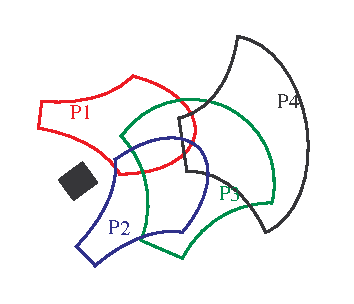
\includegraphics[width=\linewidth]{graphics/nondeter2D.eps} 

{\footnotesize (a)}
\end{minipage}
\hspace{0.05\linewidth}
\begin{minipage}{0.45\linewidth}
  \centering 
\psfrag{P1}[]{\textcolor{red}{$\CP_A$}}
\psfrag{P2}[]{\textcolor{blue}{$\CP_B$}}
\psfrag{P3}[]{\textcolor{DarkGreen}{$\CP_C$}}
\psfrag{P4}[]{$\CP_D$}
  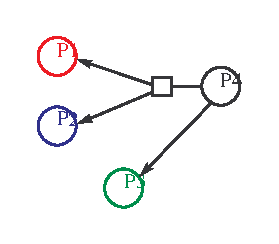
\includegraphics[width=\linewidth]{graphics/nondeterGraph.eps} 

{\footnotesize (b)}
\end{minipage}
 
\caption[Extended prepares definition]{Example of the extended
  prepares definition using iconic funnels.  a) Policy $\CP_D$
  prepares neither $\CP_A$ nor $\CP_B$, but does prepare $\CP_A \union
  \CP_B$ and $\CP_C$. b) Transition relation.  From the discrete
  planning perspective, the choice of transition from $\CP_D$ to
  $\CP_A$ or $\CP_B$ is non-deterministic; that is, it is imposed
  \emph{externally} by the closed-loop system dynamics.  The discrete
  planning method must account for either possibility.}

  \label{fig:approach_nondeter} 

\end{figure}
%% \addtolength{\floatsep}{2ex}
%% \addtolength{\textfloatsep}{2ex}
%% \addtolength{\dblfloatsep}{2ex}
%% \addtolength{\dbltextfloatsep}{2ex}

This added flexibility in the definition of prepares introduces added complexity to
the discrete transition relation encoded in the prepares graph.  Thus, the ability to
define larger goal sets via the extended prepares definition bears a cost that is
borne by the discrete planning.  The flow along a vector field is mathematically
determinate; therefore, from any initial condition within the single policy the flow
will result in a transition specific policies in the union. On the other hand, the
discrete transition relation encoded by the extended prepares relationship is an
approximation.  From the point of view of the discrete relationship, the transition
is non-deterministic, and cannot be represented by a simple graph.  The
nondeterminacy can be represented as an \emph{action} with multiple \emph{outcomes},
as shown in \refig{approach_nondeter}-b.  This representation is common with Markov
Decision Processes (MDP)~\cite{maxim_03,Wiki:MDP}.  From the perspective of the
discrete planning system, the choice of outcome is \emph{externally} imposed on the
discrete transition relation by the closed-loop system dynamics.
%once the hybrid control system choses an action based on its switching strategy.  
So long as the planning system takes each possible outcome into
account, the transition relation is valid for planning.  We will abuse
notation and continue to refer to the transition relation as a
``prepares graph'', even for the case of non-deterministic outcomes
induced by the extended prepares relationship.

%\FloatBarrier

\subsection{Policy Space Planning}
\label{sec:approach_planning}

This section highlights several issues involved in planning over a
collection of control policies that satisfy the above requirements.
Several approaches to defining switching strategies among the policies
are discussed; these approaches make use of existing discrete planning
techniques.  The discussion extends the basic partial order approach
presented in~\cite{bur_riz_kod_99}.  This thesis work enables advanced
planning techniques to be applied to systems with more complex
dynamics and constraints.

The planning takes place in the space of instantiated local feedback control
policies.  Recall from \resec{related_basicseqcomp}, that the \emph{palette} is a
collection of generic policies; that is policies with free parameters.  Policies are
\emph{instantiated} by assigning specific parameter values to a generic policy chosen
from the palette.  Given a collection of instantiated policies, which we call a
\emph{suite} of policies, planning involves defining a switching strategy among those
policies to address a given task.  The suite of policies and the switching strategy
is called a \emph{deployment}.


%% \addtolength{\floatsep}{-2ex}
%% \addtolength{\textfloatsep}{-2ex}
%% \addtolength{\dblfloatsep}{-2ex}
%% \addtolength{\dbltextfloatsep}{-2ex}
\begin{figure}[bt]
  \centering 
\begin{minipage}{0.85\linewidth}
  \centering 
\psfrag{P1}[]{\textcolor{red}{ $\CP_A$}}
\psfrag{P2}[]{\textcolor{blue}{ $\CP_B$}}
\psfrag{P3}[]{\textcolor{DarkGreen}{ $\CP_C$}}
\psfrag{P4}[]{\textcolor{black}{ $\CP_D$}}
\psfrag{P5}[]{\textcolor{blue}{ $\CP_E$}}
\psfrag{P6}[]{\textcolor{red}{ $\CP_F$}}
\psfrag{P7}[]{\textcolor{DarkGreen}{ $\CP_G$}}
\psfrag{P8}[]{\textcolor{blue}{ $\CP_H$}}
\psfrag{P9}[]{\textcolor{black}{ $\CP_I$}}
\psfrag{P10}[]{\textcolor{DarkGreen}{ $\CP_J$}}
\psfrag{P11}[]{\textcolor{blue}{ $\CP_K$}}
\psfrag{P12}[]{\textcolor{black}{ $\CP_L$}}
\psfrag{P13}[]{\textcolor{red}{ $\CP_M$}}
\psfrag{P14}[]{\textcolor{DarkGreen}{ $\CP_N$}}
\psfrag{P15}[]{\textcolor{blue}{ $\CP_O$}}
\psfrag{P16}[]{\textcolor{red}{ $\CP_P$}}
\psfrag{P17}[]{\textcolor{DarkGreen}{ $\CP_Q$}}
\psfrag{P18}[]{\textcolor{blue}{ $\CP_R$}}
\psfrag{P19}[]{\textcolor{black}{ $\CP_S$}}
\psfrag{P20}[]{\textcolor{red}{ $\CP_T$}}
\psfrag{P21}[]{\textcolor{black}{ $\CP_U$}}
\psfrag{P22}[]{\textcolor{DarkGreen}{ $\CP_V$}}
\psfrag{P23}[]{\textcolor{black}{ $\CP_W$}}
\psfrag{P24}[]{\textcolor{red}{ $\CP_X$}}
\psfrag{P25}[]{\textcolor{DarkGreen}{ $\CP_Y$}}
\psfrag{P26}[]{\textcolor{black}{ $\CP_Z$}}

  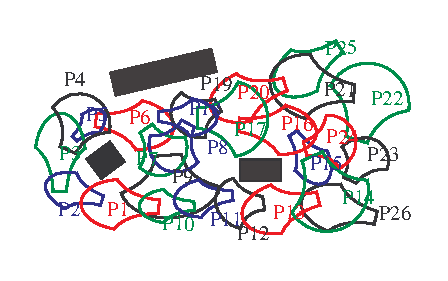
\includegraphics[width=\linewidth]{graphics/collection2D.eps} 

{\footnotesize (a)}
\end{minipage}

%\hspace{0.05\linewidth}

\begin{minipage}{0.85\linewidth}
  \centering 
\psfrag{P1}[]{\textcolor{red}{ $\CP_A$}}
\psfrag{P2}[]{\textcolor{blue}{ $\CP_B$}}
\psfrag{P3}[]{\textcolor{DarkGreen}{ $\CP_C$}}
\psfrag{P4}[]{\textcolor{black}{ $\CP_D$}}
\psfrag{P5}[]{\textcolor{blue}{ $\CP_E$}}
\psfrag{P6}[]{\textcolor{red}{ $\CP_F$}}
\psfrag{P7}[]{\textcolor{DarkGreen}{ $\CP_G$}}
\psfrag{P8}[]{\textcolor{blue}{ $\CP_H$}}
\psfrag{P9}[]{\textcolor{black}{ $\CP_I$}}
\psfrag{P10}[]{\textcolor{DarkGreen}{ $\CP_J$}}
\psfrag{P11}[]{\textcolor{blue}{ $\CP_K$}}
\psfrag{P12}[]{\textcolor{black}{ $\CP_L$}}
\psfrag{P13}[]{\textcolor{red}{ $\CP_M$}}
\psfrag{P14}[]{\textcolor{DarkGreen}{ $\CP_N$}}
\psfrag{P15}[]{\textcolor{blue}{ $\CP_O$}}
\psfrag{P16}[]{\textcolor{red}{ $\CP_P$}}
\psfrag{P17}[]{\textcolor{DarkGreen}{ $\CP_Q$}}
\psfrag{P18}[]{\textcolor{blue}{ $\CP_R$}}
\psfrag{P19}[]{\textcolor{black}{ $\CP_S$}}
\psfrag{P20}[]{\textcolor{red}{ $\CP_T$}}
\psfrag{P21}[]{\textcolor{black}{ $\CP_U$}}
\psfrag{P22}[]{\textcolor{DarkGreen}{ $\CP_V$}}
\psfrag{P23}[]{\textcolor{black}{ $\CP_W$}}
\psfrag{P24}[]{\textcolor{red}{ $\CP_X$}}
\psfrag{P25}[]{\textcolor{DarkGreen}{ $\CP_Y$}}
\psfrag{P26}[]{\textcolor{black}{ $\CP_Z$}}
\psfrag*{1}{{ $1$}}
\psfrag*{2}{{ $2$}}
\psfrag*{3}{{ $3$}}

  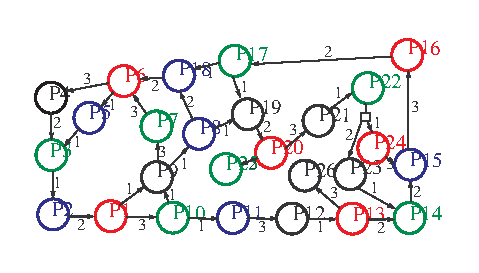
\includegraphics[width=\linewidth]{graphics/collectionGraph.eps} 

{\footnotesize (b)}
\end{minipage}

\caption[Example collection of policies and prepares graph]{Given the
  collection of iconic policies $\Lambda$ shown in (a), the discrete
  transition relation $\GL$ shown in (b) encodes the ``prepares''
  relationship between policies.  Thus the continuous behavior of the
  system is abstracted as a discrete set of transitions between policy
  domains.  Each transition shows an associated heuristic cost that
  may be used in planning.}

  \label{fig:approach_prepares} 

\end{figure}
%% \addtolength{\floatsep}{2ex}
%% \addtolength{\textfloatsep}{2ex}
%% \addtolength{\dblfloatsep}{2ex}
%% \addtolength{\dbltextfloatsep}{2ex}

To illustrate the types of planning that are possible on the discrete
prepares graph, consider the ``toy'' example shown in
\refig{approach_prepares}.  Here 26 policies are instantiated over the
workspace with three obstacles; these policies make up the suite
$\Lambda = \crl{\CP_A, \dots, \CP_Z}$.  The policy domains are shown
in \refig{approach_prepares}-a, and the associated prepares graph,
\GL, is shown in \refig{approach_prepares}-b.  The figure shows one
example of the extended prepares definition with $\CP_V \succeq
\crl{\CP_X, \CP_W}$.  Two policies, $\CP_Y$ and $\CP_Z$, do not
prepare any others.  As is generally the case, the prepares graph is
cyclic.

In the discussion that follows, some planning methods use a cost associated with each
transition to facilitate policy ordering.  In this example, a heuristic cost has been
assigned to each edge in the graph shown in \refig{approach_prepares}-b.  This
section does not address how the costs are assigned.
%, and instead assumes they are given.

In the subsequent discussion, the switching strategies are often
modeled as finite automata, with nodes and transitions between nodes.
For each node there is an associated policy that is executed upon
transition into the node.  Initially, there is a one-to-one
correspondence between nodes and policies; later, as temporal
dependencies are incorporated, the automata will have multiple nodes
that map to a single policy.  For this reason, this discussion will
enforce a distinction between a node in the automata representation
and its associated control policy.  Transitions represent switches
between policies governed by the continuous state evolution into the
domain of a policy associated with a child node; that is, the
transitions are enabled with the state enters the domain of a policy
associated with a child node.  

For transitions based on the extended prepares definition, the
transition will be associated with a non-deterministic outcome, and the
finite automata may more properly be modeled as a Markov Decision
process.  Here the transition is an action, with multiple outcomes.
The action represents a desired transition to a set of nodes
associated with the set of policies in the extended prepares.  The
transition is enables as soon as the system state enters the domain of
any policy associated with an outcome node.  This thesis will use the
term finite automata to encompass the non-deterministic outcomes.

For simple navigation to an overall goal, we assume the existence of a
single stabilizing policy, which will be referred to as the ``goal
policy.''  The node in the automaton that is associated with the goal
policy will be the termed the ``goal node.''  In some cases, where the
system has a known initial condition, references to the ``initial
policy'' and ``initial node'' are made as appropriate, where the
initial state is contained in the domain of the initial policy.

\subsection{Automata-based Planning}
\label{sec:automata}

In order to plan for higher-level task specification, including those
with the need to respond to events or respect temporal restrictions, a
more flexible planning approach is needed.  Sequence-based approaches
require replanning if the system needs to react to an event, and
order-based approaches by themselves are only suitable for single
tasks.  To address this issue, recent work has focused on
automatically synthesizing automata from a prepares
graph~\cite{belta_06,hadas_07}.

Combining policy composition with automata synthesis leverages the strengths of
control theoretic and computer science approaches.  Control theoretic approaches
offer provable guarantees over local domains; unfortunately, the control design
requires a low-level specification of the task.  In contrast, discrete planning
advances from computer science offer the ability to specify more general behaviors,
which may react to environmental changes, and generate verifiable solutions at the
discrete level; discrete planning lacks the continuous guarantees and robustness
offered by feedback.  Synthesizing an automaton that governs the execution of the
local feedback policies provides the benefits of both feedback and discrete planning,
while mitigating the drawbacks.  These automata synthesis tools specify behaviors in
terms of linear temporal logic (LTL) operations on the prepares graph nodes.  LTL
combines the standard Boolean logic operators, such as `AND',`OR', and `NOT', with
temporal operators such as 'ALWAYS' and 'NEXT'~\cite{Emerson}.

Kress-Gazit \ea~\cite{hadas_07} have developed an automaton synthesis tool that use
specifications encoded in a subset of the full LTL that describe behaviors on the
prepares graph generated by the work in this thesis.  The approach allows both
discrete inputs and discrete outputs to be specified.  The discrete inputs are sensed
by the robot, and the discrete outputs trigger actions, such as sound an alarm.  This
allows the system to change high-level behavior-based on discrete events, which
allows the system to react to environmental changes in a guaranteed manner.
Given a specification and prepares graph, the synthesis process either extracts an
automaton that satisfies the specification, or shows that the specification is not
realizable on the prepares graph.  Transitions in the automaton are governed by the
transitions between policy domains and the discrete events sensed by the
robot~\cite{dcchkg_07}.  Thus, the combination of automata and continuous feedback
control policies allows high-level specifications to be satisfied by executing the
continuous feedback control policies.  The work in this thesis has enabled these
approaches to be applied to more complex systems.


% Some LTL operators are
% shown in Table~\ref{table:LTL_ops}.
% \begin{table}
% \caption{Some standard LTL operators.}
% \centering
% \begin{tabular}{|c|c|}
% \hline
% `NOT' & $\NOT$\\
% `AND'&$\AND$\\
% `OR' &$\OR$\\
% `IMPLIES'& $\IMPLIES$\\
% `IF AND ONLY IF' & $\IFF$\\
% `NEXT' & $\NEXT$\\
% `ALWAYS' & $\ALWAYS$\\
% `EVENTUALLY' & $\EVENTUALLY$\\
% `UNTIL' &$\UNTIL$\\
% \hline
% \end{tabular}
% \label{table:LTL_ops}
% \end{table}


%% \addtolength{\floatsep}{-2ex}
%% \addtolength{\textfloatsep}{-2ex}
%% \addtolength{\dblfloatsep}{-2ex}
%% \addtolength{\dbltextfloatsep}{-2ex}
\begin{figure}[bt]%
  \centering 
\begin{minipage}{0.85\linewidth}
  \centering 
\psfrag{S}[]{$S$}
\psfrag{E}[]{Event `EV'}
\psfrag{G}[]{$G$}

  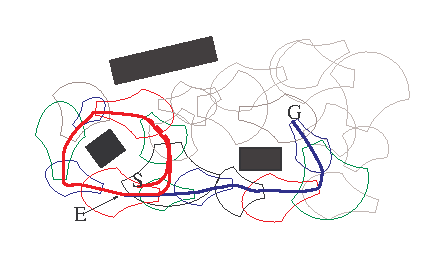
\includegraphics[width=\linewidth]{graphics/automaton2D.eps} 

{\footnotesize (a)}
\end{minipage}
%\hspace{0.05\linewidth}

\begin{minipage}{0.85\linewidth}
  \centering 
\psfrag{P1}[]{\textcolor{red}{ $\CP_A$}}
\psfrag{P2}[]{\textcolor{blue}{ $\CP_B$}}
\psfrag{P3}[]{\textcolor{DarkGreen}{ $\CP_C$}}
\psfrag{P4}[]{\textcolor{black}{ $\CP_D$}}
\psfrag{P5}[]{\textcolor{blue}{ $\CP_E$}}
\psfrag{P6}[]{\textcolor{red}{ $\CP_F$}}
\psfrag{P7}[]{\textcolor{DarkGreen}{ $\CP_G$}}
\psfrag{P8}[]{\textcolor{blue}{ $\CP_H$}}
\psfrag{P9}[]{\textcolor{black}{ $\CP_I$}}
\psfrag{P10}[]{\textcolor{DarkGreen}{ $\CP_J$}}
\psfrag{P11}[]{\textcolor{blue}{ $\CP_K$}}
\psfrag{P12}[]{\textcolor{black}{ $\CP_L$}}
\psfrag{P13}[]{\textcolor{red}{ $\CP_M$}}
\psfrag{P14}[]{\textcolor{DarkGreen}{ $\CP_N$}}
\psfrag{P15}[]{\textcolor{blue}{ $\CP_O$}}
\psfrag{IC}[]{IC}
\psfrag{NG}[cB]{$\neg\,\mrm{EV}$}
\psfrag{GD}[lt]{EV}

  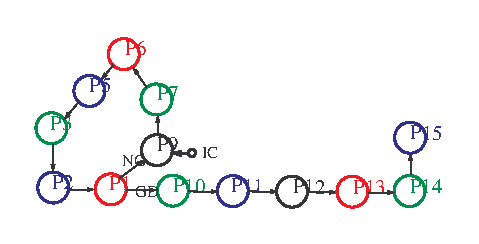
\includegraphics[width=\linewidth]{graphics/automatonGraph.eps} 

{\footnotesize (b)}
\end{minipage}

\caption[Automata-based planning]{ Automata-based planning allows for
  the system to react to local conditions while satisfying a given
  specification.   Figure (a) shows portions of the path taken while satisfying
  the automaton shown in (b).  }

  \label{fig:approach_automaton} 

\end{figure}
%% \addtolength{\floatsep}{2ex}
%% \addtolength{\textfloatsep}{2ex}
%% \addtolength{\dblfloatsep}{2ex}
%% \addtolength{\dbltextfloatsep}{2ex}

%\clearpage % just for this run

Returning to the example of \refig{approach_prepares}, we wish to specify that the
robot patrol the lower left obstacle until an event is seen, and then goes to a
particular station.  The first part, ``patrol
the lower left obstacle by visiting areas `F' and `A', until an event `EV' at `A' is
seen.''  
%, is given in LTL by $\prl{\prl{\ALWAYS\EVENTUALLY \CP_F \AND \ALWAYS\EVENTUALLY
%    \CP_A }\UNTIL \prl{\CP_A \AND \mrm{EV}}}$\footnote{There are two subtleties with this specification.  Due to
%  the formalism of the UNTIL operator, this particular formula is only
%  valid if ${\CP_A \AND \mrm{EV}}$ eventually becomes true; that is
%  the event eventually happens.  Also, we assume policy 'O' stops in
%  the goal set.}.  
After seeing the event, ``go to 'O', sound an  and stay put.''
% is given by
%$\ALWAYS\prl{\prl{\CP_A \AND \mrm{EV}} \Rightarrow \EVENTUALLY \CP_O}  \AND
%\ALWAYS\prl{\CP_O \Rightarrow \NEXT \CP_O}$.  At 'O', ``sound an alarm'' is encoded
%by $\ALWAYS\prl{\CP_O \Rightarrow `ALARM'}$.  All of these should be true for the
% complete system behavior, so they are combined to give the temporal logic formula 
% \begin{equation}
% \bba{c}
% \prl{\prl{\ALWAYS\EVENTUALLY \CP_F \AND \ALWAYS\EVENTUALLY
%     \CP_A }\UNTIL \prl{\CP_A \AND \mrm{EV}}}\\
% \AND\\
% \ALWAYS\prl{\prl{\CP_A \AND \mrm{EV}} \Rightarrow \EVENTUALLY \CP_O} \\
% \AND\\
% \ALWAYS\prl{\CP_O \Rightarrow \NEXT \CP_O} \\
% \AND\\
% \ALWAYS\prl{\CP_O \Rightarrow `ALARM'}
% \eba\,.
% \label{eqn:approach_LTL_spec}
% \end{equation}
\refig{approach_automaton} shows an example of an automaton whose execution satisfies
this behavior.  %Automata synthesis is an active research area.
%The remainder of this section focuses on a specific approach used in conjunction with
%this thesis.
 
There are several down sides to the current automata synthesis
approaches.  First, these current approaches do not consider
transition costs.  Thus, a heuristic cost associated with invoking a
more complex policy is not taken into consideration by the current
synthesis tools.  Second, because the automaton does not use all of
the policies in the collection, some robustness to disturbance is
lost.  In \resec{planning}, we present one approach to combining the
automata synthesis with order-based planning to improve the robustness
of the automaton.



\subsection{Some Text that was commented out in my thesis}
\label{sec:approach_extra_text}


The automaton then governs the policy switching behavior according to the discrete
events detected by sensors and the current state of the robot. v

 %is a game played between the robot and its environment.  The
 %environment controls the discrete inputs, while the robot has control of its
 %iscrete outputs and the policies chosen according to the prepares
 %graph $\GL$.  The robot wins the game if a sequence of policies and
 %discrete outputs can satisfy a given specification regardless of the
 %inputs defined by the environment.

 The rules of the game specify both initial conditions and a transition
 relation defining the moves that the robot and environment can
 make\footnote{The following text is derived from a joint
   paper~\cite{dcchkg_07} with Hadas Kress-Gazit and George J.
   Pappas.}.  One of the rules is that all transitions must obey the
 prepares graph $\GL$.  The winning condition, $\sigma$, for the game
 is a specification given as a fragment of LTL.
 %Generalized Reactivity(1) formula formula $\sigma$. 
 The way the game is played is that at each step, first the environment
 makes a transition according to its transition relation, and then the
 system makes its own transition.  If the environment can falsify
 $\sigma$, then the environment wins and the desired behavior is
 unrealizable.  If the system can satisfy $\sigma$ no matter what the
 environment does, the system wins and the synthesis
 algorithm~\cite{piterman_06} can extract an automaton.  The extracted
 automaton defines a possible, but not necessarily unique, switching
 strategy for the collection of policies such that the system can react
 to inputs and satisfy a high-level specification.

  The input to the algorithm is an LTL formula $\varphi$ that encodes
  the rules of the game in the following form:
  $$\varphi\; =\; (\varphi_e \Rightarrow \varphi_s)$$
  $\varphi_e$ is an assumption about the inputs, and thus about the
  behavior of the environment, and $\varphi_s$ represents the desired
  behavior of the system.  More specifically,
  $$\varphi_e =\varphi_i^e \wedge \varphi_t^e \wedge
  \varphi_g^e $$
  $$\varphi_s =\varphi_i^s \wedge \varphi_t^s \wedge
  \varphi_g^s$$
  where

  \begin{itemize}
  
  \item $\varphi_i^e$ - Boolean formulas in the discrete inputs
    describing the initial condition of the environment
  
  \item $\varphi_t^e$ - Assumptions on how the environment can change;
    that is its allowable transitions.  $\varphi_t^e$ consists of a
    conjunction of formulas of the form $\Box B_i$ where each $B_i$ is a
    boolean formula constructed from sub-formulas in the sets of
    discrete inputs, discrete outputs, and nodes in $\GL$.  Intuitively,
    $\varphi_t^e$ constrains the next possible input values based on the
    current input and system state.
  
  \item $\varphi_i^s$ - Boolean formulas in the discrete outputs and
    nodes in $\GL$ describing the initial condition of the system
  
  \item $\varphi_t^s$ - Constraints on the moves the system can take. It
    consists of a conjunction of formulas of the form $\Box B_i$ where
    each $B_i$ is a boolean formula over the current discrete outputs,
    current node in $\GL$, current input, and the next input (since the
    environment moves first).  These constrain the next discrete output
    and node in $\GL$; these formulas encode the prepares relationships
    specified in $\GL$.
  \item $\varphi_g^e$, $\varphi_g^s$ - Represent goal assumptions for
    the environment and desired goal specifications for the system
    respectively. Both formulas consist of a conjunction of formulas of
    the form $\Box \Diamond B_i$, where each $B_i$ is a boolean formula.
  \end{itemize}

  Translating this formula to a game, the initial condition is
  $\varphi_i^e \wedge \varphi_i^s$, the transition relations for the
  players are $\varphi_t^e$ and $\varphi_t^s$, and the winning condition
  is $\sigma=(\varphi_g^e\;\Rightarrow\; \varphi_g^s)$.  Note, there are
  two ``ways'' for the system to win. It wins if either $\varphi_g^s$ is
  satisfied, i.e. the system reaches its goals, \textbf{or}
  $\varphi_g^e$ is falsified. The later case implies that if the
  environment does not satisfy its goals (invalid input), then a correct
  behavior of the system is no longer guaranteed.

  Returning to the example above, each behavior is encoded for the input
  formulas.  For the environmental transitions, we have $\varphi_t^e =
  \ALWAYS\prl{\NOT \CP_A \Rightarrow \prl{\NEXT \mrm{EV} \Leftrightarrow
      \mrm{EV}}}$; that is, EV can only change in the domain of $\CP_A$.
  For the system transitions, $\varphi_t^s = \ALWAYS\prl{\CP_O
    \Rightarrow \NEXT\CP_O} \AND \GL \AND \varphi_\mrm{alert}$.  The
  first part encodes stay at $\CP_O$ once you get there; $\GL$ is the
  prepares graph encoded in LTL.  For example, node $\CP_F \in \GL$
  would be encoded as $\ALWAYS \CP_F \Rightarrow \prl{\NEXT \CP_F\ \OR \ 
    \NEXT \CP_D\ \OR \ \NEXT\CP_E}$.  Note the self transition is due to
  the fact that the system takes finite time to traverse the domain of a
  given policy.  The last part of $\varphi_t^s$ encodes a discrete
  output that raises an alert in response to the event after reaching
  $\CP_O$; $\varphi_\mrm{alert}$ is given by
  \[
  \bba{c}
  \ALWAYS\prl{\prl{\NOT\NEXT\CP_O} \Rightarrow \prl{\NEXT \mrm{ALERT}
      \Leftrightarrow \mrm{ALERT}}}\\\AND\\\ALWAYS\prl{\NEXT\CP_O \Rightarrow
    \NEXT\mrm{ALERT}}
  \eba
  \, ,
   \ALWAYS\prl{\prl{\NOT\NEXT
      \mrm{EV}} \Rightarrow \prl{\NEXT \mrm{ALERT} \Leftrightarrow
      \mrm{ALERT}}}\\\AND
  \]
  $\varphi_\mrm{alert}$ encodes that the ALERT output cannot change
  except at $\CP_O$ after the event EV.  For the initial conditions,
  $\varphi^s_i = \NOT\mrm{ALERT} \AND \CP_I$ and $\varphi^e_i = \NOT
  EV$; that is we start in $\CP_I$ without an alert set and the event
  has not occurred.  The environment goal is $\varphi_g^e = \mrm{true}$.
  The system goal $\varphi^s_g = \prl{\ALWAYS\EVENTUALLY\prl{\CP_F \OR
      \mrm{EV}}\ \AND\ \ALWAYS\EVENTUALLY\prl{\CP_A \OR \mrm{EV}}\ \AND
         \ \ALWAYS\EVENTUALLY\prl{\CP_O \OR \NOT \mrm{EV}}}$.


 For a given prepares graph and specification, the synthesis algorithm
 has the potential to evaluate $\mid\!\!\GL\!\! \mid 2^{\prl{n+o}} L$
 nodes, where $\mid\!\!\GL\!\!\mid$ is the number of nodes in the prepares
 graph, $n+o$ is the total number of discrete inputs and outputs, and
 $L$ is the number of liveness conditions.  In the example from
 \refig{approach_automaton}, $\mid\!\!\GL\!\!\mid = 26$, $n = 1$, $o=1$,
 and $L = 3$, where the liveness conditions are visit $\CP_A$, $\CP_F$,
 and $\CP_O$.  This gives a potential of $26*4*3=312$ nodes.  As can be
 seen from the automaton in \refig{approach_automaton}, the actual
 number of required nodes is much less.  The synthesis tools use model
 checking technology to address the state explosion problem during
 synthesis~\cite{hadas_07,piterman_06}.

 The complexity of the automaton synthesis grows with the number of
 policies in the prepares graph, the number of discrete inputs and
 outputs, and the number of ``liveness conditions.''  Formally, the
 synthesis algorithm has the potential to evaluate $\mid\!\!\GL\!\!
 \mid 2^{\prl{n+o}} L$ nodes, where $\mid\!\!\GL\!\!\mid$ is the number
 of nodes in the prepares graph, $n+o$ is the total number of discrete
 inputs and outputs, and $L$ is the number of liveness conditions.  In
 the example from \refig{approach_automaton}, $\mid\!\!\GL\!\!\mid =
 26$, $n = 1$, $o=1$, and $L = 3$, where the liveness conditions are
 visit $\CP_A$, $\CP_F$, and $\CP_O$.  This gives a potential of
 $26*4*3=312$ nodes.  As can be seen from the automaton in
 \refig{approach_automaton}, the actual number of required nodes is
 much less.  The synthesis tools use model checking technology to
 address the state explosion problem during
 synthesis~\cite{hadas_07,piterman_06}.



\subsection{Summary}
\label{sec:approach_summary}

This chapter has introduced two extensions to the basic sequential composition
technique.  First, flow-through policies are introduced, which allow the system to
encode natural behaviors for nonholonomic systems.  Second, the prepares definition
is extended to allow a policy to prepare a set of policies.  This extension provides
more flexibility in instantiating the local policies, but complicates the discrete
planning.  The impact of this change on the planning is discussed.

The chapter discusses the properties that are necessary for composable policies.  In
addition to policies that that respect the system constraints, the policy domains
must be completely contained in the free state space and conditionally invariant.
The vector field flow induced by the closed-loop policy must converge to a well
defined goal set in finite time.  Additionally, the policies should have simple and
efficient inclusion tests to allow the approach to be executed in real time.  Any
policy with these properties can be deployed in our hybrid control framework.

The chapter discusses approaches to planning in the space of instantiated policies.
Three basic approaches are presented: sequence-based, order-based, and
automata-based.  A ``toy'' example highlights the differences between the approaches.
\resec{planning} discusses the relative strengths and weaknesses of each approach.
In general, order-based and automata-based approaches are preferred over the
sequence-based approaches for reasons of robustness and flexibility.



\section{Experimental Setup}
\label{sec:setup}

{\large  Describe the experimental setup including robot model, policy design and deployment.}


This section  demonstrates the coupled planning and control approaches
advocated in this thesis; experiments and simulations validate the
approaches discussed in \resec{approach}.  The experiments are
designed to demonstrate the automata-based planning approaches using
the policies developed in`\cite{dcc_thesis}.  The approach is applied
to real systems that exhibit the imperfections and model uncertainty
of real world applications, operating in confined environments.  The
results demonstrate that the combination of simple feedback control
policies with automata synthesis techniques allows complex behaviors
to emerge; unlike other behavior-based approaches~\cite{brooks_86},
these emergent behaviors are guaranteed to induced the desire global
behavior.  The experiments also exhibit the robustness of feedback
control to model uncertainty and disturbances.  In spite of the
overall success, several issues arise during the testing.  We discuss
these issues, how they impact the relative strengths and weaknesses of
the different approaches, and present our methods of addressing the
issues.


\subsection{`LAGR' Robot Experiments}
\label{sec:lagr_total_order}

The previous experiments did not have integrated localization, which limits their
practical value.  Using pure dead reckoning makes the experiment too much like a
simulation, as the hybrid control system is not subject to disturbances due to
localization error and correction.  To address this shortcoming, a second set of
order-based experiments uses a robot equipped with an integrated vision-based
localization system.  This allows the hybrid control approach developed in this
thesis to be evaluated in an integrated system.

\begin{figure}[bt]
  \centering 
   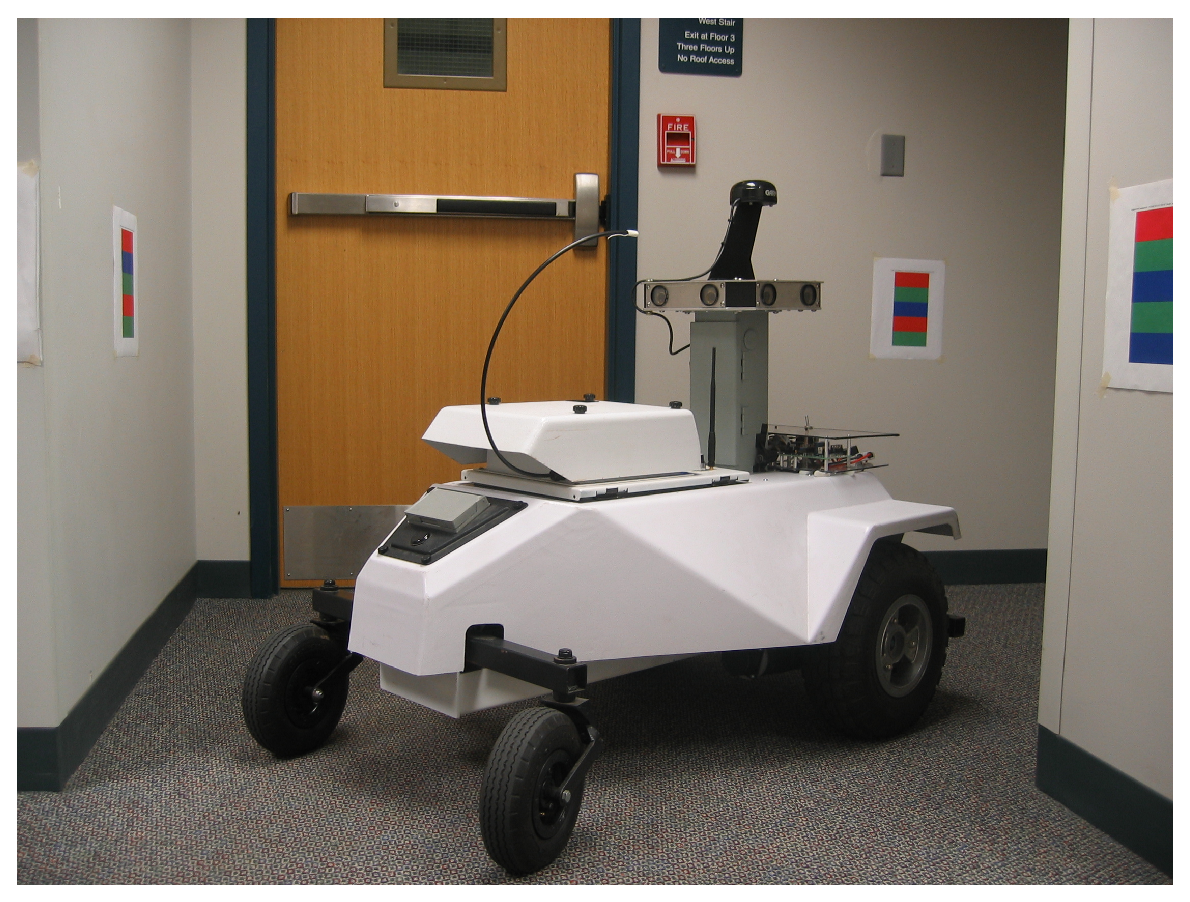
\includegraphics[width=\linewidth]{graphics/Lagr_14Oct07_008.eps}

   \caption[`LAGR' robot navigating a corridor.]{`LAGR' robot navigating a corridor.
     Three color-coded landmarks, which are used by the vision based localization
     system, are visible in the image.}
   \label{fig:lagr_nook}
\end{figure}

In the next set of experiments, we use the `LAGR' robot shown in \refig{lagr_nook}
because it has four pairs of stereo cameras to perform vision based localization relative
to known landmarks placed in the environment; the landmarks are color coded as shown
in \refig{lagr_nook}.  The localization system uses an extended Kalman filter to
update the pose estimate based on measurements of range and bearing to the identified
landmarks.  The system is now subject to disturbances based on jumps in the pose
estimate as new landmarks come into view.


%% \addtolength{\floatsep}{-2ex}
%% \addtolength{\textfloatsep}{-2ex}
%% \addtolength{\dblfloatsep}{-2ex}
%% \addtolength{\dbltextfloatsep}{-2ex}
\begin{figure}[bt]
\begin{center}
\vspace{0.25ex}
\begin{minipage}[b]{0.98\linewidth}
\centering
\begin{minipage}[b]{\linewidth}
\begin{minipage}[c]{0.45\linewidth} % A minipage that covers half the page
  \centering
  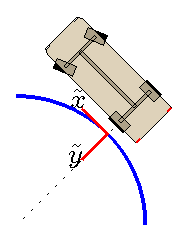
\includegraphics[width=0.4\linewidth]{graphics/policy_curve.eps} 
\end{minipage}
\hspace{0.05\linewidth} % To get a little bit of space between the figures
\begin{minipage}[c]{0.45\linewidth}
  \centering 
  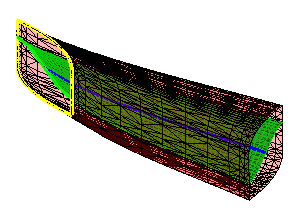
\includegraphics[width=0.7\linewidth]{graphics/policy_tube.eps}
\end{minipage}
\end{minipage}

\vspace{0.5ex}

\begin{minipage}[b]{\linewidth}
\begin{minipage}[t]{0.48\linewidth} % A minipage that covers half the page
\centering

   {\footnotesize a) Workspace path with local frame defined }

\end{minipage}
\hspace{0.02\linewidth} % To get a little bit of space between the figures
\begin{minipage}[t]{0.48\linewidth}
  \centering   

  {\footnotesize b) Cell boundary and ``sliding'' control surface.}  

\end{minipage}

\end{minipage}
\end{minipage}
\caption[Path following style policy]{Control policy based on path following control
  law given in \cite{vsc_path_following}.}
\label{fig:nonholo_PF_policy}
\end{center}
\end{figure}
%% \addtolength{\floatsep}{2ex}
%% \addtolength{\textfloatsep}{2ex}
%% \addtolength{\dblfloatsep}{2ex}
%% \addtolength{\dbltextfloatsep}{2ex}

These experiments are carried out with `\PF' style control
policies~\cite{dcc_thesis,conner_09}.  The policy design is based on a
variable structure control approach to path following, which gives the
policy its `PF' name~\cite{vsc_path_following}.  The `PF' policies are
based on workspace path segments, which are used to define a
parameterized cell in pose space.  The path segment is lifted to a
curve in pose space by considering the orientation of the path tangent
as the desired system orientation, with the goal set center at one end
of the pose space curve.  A `tube' is defined around the pose space
curve to define the cell boundary.  \refig{nonholo_PF_policy} shows an
example of this cell.  The PF policy defines a ``sliding'' control
surface within the cell boundary tube.

For a given robot model, the policy defines a control strategy that
causes the system to steer toward the sliding surface, then along the
sliding surface towards the pose space curve and the goal set center.
For kinematic systems, the sliding surface defines a velocity
constraint at each pose; the constraint is then mapped to a constraint
on the input space, where a simple optimization is used to chose a
valid input.  See~\cite{dcc_thesis} or~\cite{conner_09} for details.


In addition to the goal set center, the policy free parameters include
the width of the tube, the curvature of the workspace path, arc length
of the path segment, and shape of the sliding surface.  Valid values
of the free parameters, that is values that induce composable
behavior, are limited by the input constraints and specific robot
system model.  Thus, the composability requirements must be verified
for a given set of parameter values


For valid parameters, the induced dynamics cause
the system to converge to the pose space curve while remaining in the
cell until the system passes the designated end point and flows out of
the cell via the goal set in finite time.
The \PF policies are natural for specifying motion in corridors and around tight corners. 

{\large get rid of the ``instead of'' contrast, and give very brief introduction to policy definition.}

Instead of the manual instantiation approach taken with the previous experiments,
these \PF policies are instantiated using the cache and reference point approach
discussed in \resec{nonholo}.  A total of 313 policies are systematically defined in
the cache; 156 forward, 156 reverse, and one special `Halt'.  These policies include
various widths, lengths, and arc radii.  Each policy in the cache is associated with
a one of thirteen bounded input sets; the inputs for each policy are taken from its
associated input set.  See \reapp{robots} for specific details about the input sets.
The input sets include sets for straight PF policies and arc based PF policies.  Both
forward and reverse sets are associated with each group, as are aggressive and
cautious sets.  The sets for straight policies allow less aggressive steering, while
those for tight turns use a cautious forward speed and more aggressive steering.  By
matching the input set to a particular policy, the feedback is tuned to the local
conditions.  Even though the robot is capable of zero-radius turns, the input sets
are constrained to exclude zero-radius turns; this approximates the behavior of more
constrained systems such as cars, and provides a greater challenge to the hybrid
control approach.

%The policies are grouped so that only the longest policy is
%instantiated at a given reference point.  Longer policies dominate the
%shorter policies; that is they completely contain the domain of
%shorter policies.

\begin{figure}[bt]
  \centering 
   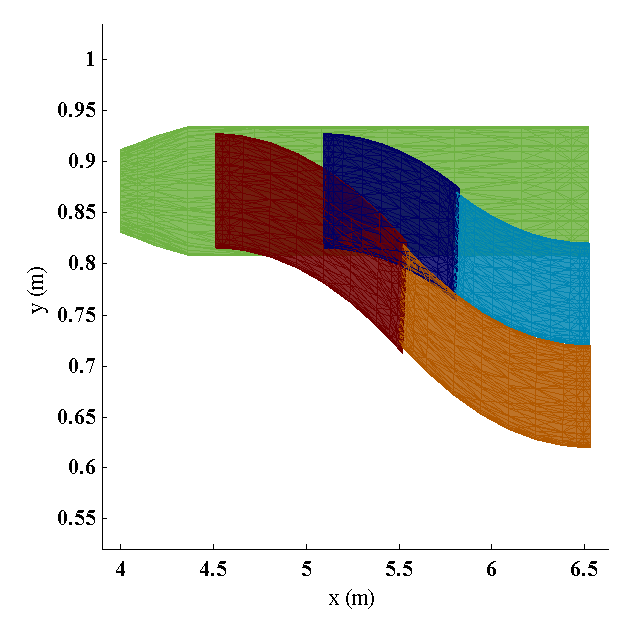
\includegraphics[width=0.55\linewidth]{graphics/lagr_meta_detail.eps}

   \caption[`LAGR' meta-policies.]{An example meta-policy that uses five \PF
     style policies to move three lanes coming from the right into a
     single lane exiting to the left.  The policies are shown
     projected into workspace.  To enhance the detail, the figures
     axes are not equal.}
   \label{fig:lagr_meta_detail}
\end{figure}

In the demonstrations here, the robot maneuvers about a hallway with
long thin corridors; therefore, it makes sense to instantiate the
policies in ``lanes.''  That is, the policies are instantiated in
straight lines running the length of the hallways; the lines of
policies are analogous to lanes on a highway.  

To further simplify policy instantiation and planning, some local policies are
grouped into meta-policies.  \refig{lagr_meta_detail} shows a meta-policy associated
with taking the system from one of three lanes entering from the right and moving the
system to the top most lane exiting to the left.  The meta-policy defines an
order-based switching strategy between its component policies, which are defined with
respect to a common reference point.  %Some cache policies are
%specifically defined such that they connect together to induce a lane
%change maneuver, as shown in \refig{lagr_meta_detail}, between evenly
%spaced lanes.
A meta-policy is instantiated by instantiating its component policies relative to its
reference point; the meta-policy can only be instantiated if all of its component
policies are collision free relative to a specified reference point in the free pose
space.  \refig{lagr_meta} shows the component policies to scale, along with the
expanded cells defined by the robot body size and shape.

\begin{figure}[bt]
 \begin{center}
 \begin{minipage}[b]{\linewidth}
 \begin{minipage}[b]{0.45\linewidth}
  \centering 
  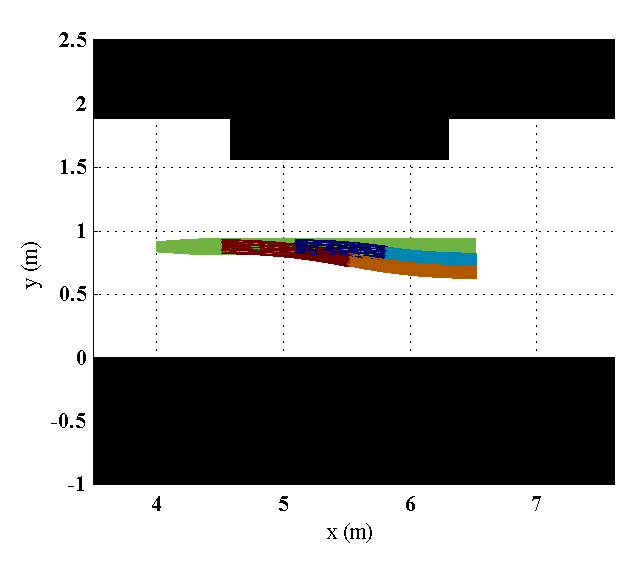
\includegraphics[width=\linewidth]{graphics/lagr_meta.eps}

  {\scriptsize a) Meta-policy projected into workspace}

 \end{minipage}
 \hspace{0.03\linewidth} % To get a little bit of space between the figures
 \begin{minipage}[b]{0.45\linewidth}
   \centering 
   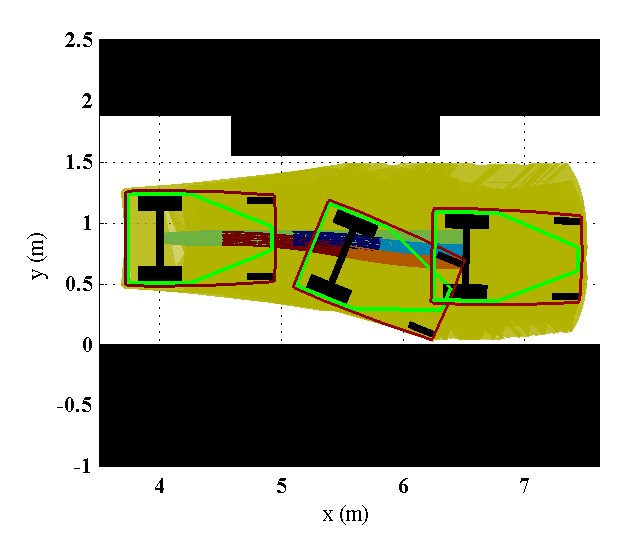
\includegraphics[width=\linewidth]{graphics/lagr_meta_padded.eps}

   {\scriptsize b) Expanded meta-policy showing body extent in
     workspace}

 \end{minipage}
 \end{minipage}
 
 \caption[Example meta-policy for `LAGR' experiments]{Example meta-policy used for
   LAGR experiments.  The meta-policy domains are shown relative to obstacles in the
   environment in the proper scale.  The figure on the right shows the body extent
   into the workspace for this meta policy.  Three robots are shown at various poses
   on the cell boundaries; the robots use a bounding polygon for calculating the body
   extent. }
  \label{fig:lagr_meta}
\end{center}
\end{figure}

While the component policies could be instantiated individually to accomplish the
same task, meta-policies simplify the deployment by grouping similar behaviors.  For
planning purposes, the meta-policy is treated as a single node in the prepares graph.
Furthermore, the meta-policies can allow manual verification of the prepares
relationships.  This can allow policies that cover the goal set, but do not all
contain the goal set center, to be prepared as a group; this removes the restrictions
of \resec{prepares_graph} for automated verification.  By design, the meta-policies
only allow designated component policies to be prepared.  This affords the designer
more control over the meta-policy behavior by allowing normally unused component
policies to be added for robustness, without including them in the prepares graph
used for planning.  These component policies can only be active after the meta-policy
becomes active.


Several meta-policies are defined based on needed motion in the
hallways.  In addition to the ``lane change right'' meta-policy,
meta-policies for ``lane change middle'' and ``lane change left'' are
defined.  Given the narrowness of the hallways, only three lanes
spaced 0.1 meters apart are defined in most corridors.  The lanes are
defined in the forward direction along the length of the corridor.
Several meta-policies associated with turning corners are defined,
including both ``left turn'' and ``right turn''.  Many of the hallways
were so narrow that a simple arc could not navigate the hallways;
therefore, two different meta-policies induce K-turn motions in the
narrow hallways.  Two additional meta-policies are defined to navigate
a small ``nook'' in the center of the region.
% \refig{lagr_nook} shows the robot navigating this nook.  When the robot is in the
% nook, it is halted by a special policy that is prepared by the incoming meta-policy;
% the halt policy prepares a meta-policy that exits the nook.


% \refig{lagr_k_turn} shows actual data from a K-turn executed by the robot
% during an experiment.  In this case, the behavior is encoded in the meta-policy by
% design, where the behavior emerged as a consequence of discrete planning in the
% Deminer experiments.

% \begin{figure}[bt]
%   \centering 
%    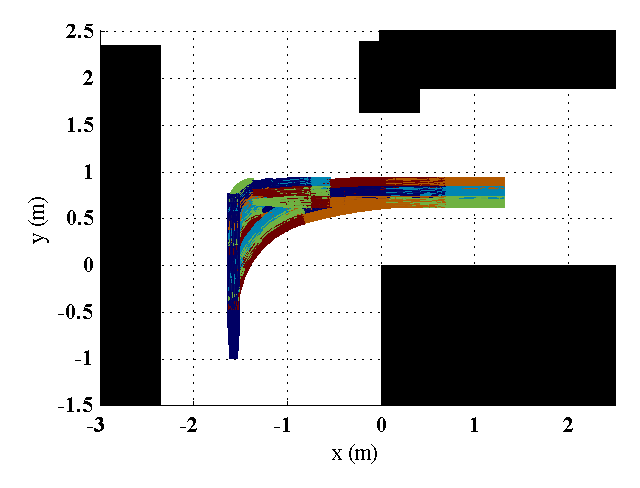
\includegraphics[width=0.55\linewidth]{graphics/lagr_meta_turn.eps}

%    \caption[`LAGR' left turn meta-policy]{Meta-policy used to turn 3 lanes left.}
%    \label{fig:lagr_meta_left}
% \end{figure}

% \refig{lagr_meta_left} shows an example left turn.  The turn
% meta-policies include simple arcs of various radii to blend three
% lanes into one orthogonal lane.  To improve robustness, the turning
% policies include both short radius turns and longer radius turns.  The
% long radius arcs blend with the short radius turns to provide a
% transition from straight motion to turning motions.

%%\FloatBarrier



% \begin{figure}[bt]
%   \centering 
% \begin{minipage}[b]{\linewidth}
% \begin{minipage}[b]{0.30\linewidth}
%   \centering 
%    \includegraphics[width=\linewidth]{graphics/total_order_K_turn_F1.eps}

%  {\scriptsize a) Approaching K-turn}

% \end{minipage}
% \hspace{0.03\linewidth} % To get a little bit of space between the figures
% \begin{minipage}[b]{0.30\linewidth}
%   \centering 

%   \includegraphics[width=\linewidth]{graphics/total_order_K_turn_R1.eps}

%  {\scriptsize b) Executing reverse motion } 

% \end{minipage}
% \hspace{0.03\linewidth} % To get a little bit of space between the figures
% \begin{minipage}[b]{0.30\linewidth}
%   \centering 

%   \includegraphics[width=\linewidth]{graphics/total_order_K_turn_F2.eps}

%  {\scriptsize b) Departing K-turn } 

% \end{minipage}
% \end{minipage}

% \caption[`LAGR' robot executing K-turn]{Plot of data from actual
%   robot experiment as the robot executes a K-turn in the upper
%   hallway.  The K-turn is automatically induced by the composition of
%   policies based on simple arcs and straight path segments. }
%    \label{fig:lagr_k_turn}
% \end{figure}


The meta-policies are implemented in a modular fashion that makes the planning and
execution transparent to the robot executive.  When testing for inclusion before
becoming active, the meta-policy only tests those component policies designated as
inlets for the prepares definition.  Once the meta-policy becomes active, all
component policies are tested using the internal ordering; that is, the inclusion
test resorts to a total order search over component policies if necessary once the
current node is associated with the meta-policy.  This approach provides robustness
to the meta-policy, while given the designer control over when the meta-policy is
allowed to become active initially.

The lane change meta-policies are instantiated at regular intervals along evenly
spaced lanes in the corridors.  The component policies in the lane-change
meta-policies are associated with input sets that have positive forward velocity.
Turn and K-turn meta-policies are instantiated in a way that they are prepared and
prepare the basic lane policies at the appropriate junctions.  In addition to the
meta-policies, a few 180 degree arcs are used in the larger central hallway to allow
continuous turns.  By design, according to the instantiated policies, the robot is
only allowed to reverse motion in certain spots through the use of a K-turn maneuver
or 180 degree arc in the central corridor.  Otherwise, the robot must travel in a
loop.


The use of meta-policies reduces the total number of nodes in the
prepares graph that is used for planning.  In this case, a total of
309 meta-policies and 86 individual policies are deployed in the
environment.  Thus, the prepares graph used for planning has only 395
nodes, compared to the grand total of 2846 \PF policies that are
instantiated in the environment.  The grand total includes both
individual and meta-policy components.  The policy suite includes 3155
policies, the 2846 \PF policies and 309 meta-policies.

The robot software executive functions the same as with the Deminer
experiments.  The planning takes place over the 395 nodes in the
prepares graph.  During execution, when a meta-policy becomes active,
it is treated as a switched hybrid control policy in its own right;
the component policies are activated according to the meta-policies
local ordering.  On the executive level, the meta-policy remains
active until the state enters the domain of a child node of the
ordering, or exits the domain of all policies in the meta-policy's
collection of component policies.

% In spite of the limitations of the LAGR robot, the order-based hybrid control policy
% robustly addressed the coupled navigation and control problem in most cases.  For single navigation
% tasks, the order-based approach to generating a hybrid control policy %based on the
% %composition of local control policies 
% proves reliable.

% \begin{comment}


% \subsection{Automata-based Planning}
% \label{sec:planning_automata}

% %Automata are more flexible than sequence-based approaches because they
% %allow the hybrid control system to react to changes in the environment
% %encountered during run time.  
% Like sequence-based approaches, automata-based switching strategies are capable of
% addressing multiple tasks; however, automata have the added advantage of changing
% behaviors during runtime based on gathered information without requiring re-planning.
% Combining the policy composition approach advocated in this thesis with automaton
% synthesis tools such as those of~\cite{hadas_07} enables a constructive approach to
% building a hybrid control policy whose continuous execution satisfies high level
% specifications, while enabling the constrained system to react to environmental
% changes.

% This section presents several experiments and simulations using the synthesis
% approach given in~\cite{hadas_07}.  As discussed in \resec{fully}, \cite{hadas_07}
% uses a disjoint workspace decomposition and adjacency graph to choose policies based
% on our fully actuated policies for idealized systems.  In contrast, this section
% defines the specifications and automata synthesis in terms of the prepares graph.
% This approach is more flexible because it can be applied to constrained systems, and
% allows for overlapping policy domains.

% The section presents two examples.  The first uses the LAGR robot and policies from
% \resec{lagr_total_order}; both simulations and experiments are discussed.  The second
% demonstration uses \PF policies with an Ackermann steered vehicle to demonstrate
% complex traffic behaviors in simulation.  The latter presentation includes a
% discussion of using this approach as the basis for a decentralized multi-agent
% control system.

% \subsection{`LAGR' Robot Experiments}
% \label{sec:lagr_automaton}

% The first example is termed the ``timid night watchman.''  The LAGR robot is tasked
% with patrolling office corridors by visiting four checkpoints in turn.  If an
% intruder is detected, as indicated by a binary sensor called `Intruder', the robot is
% to ``run and hide'' in the small nook near the workspace center; after the intruder
% is gone, the robot should resume patrolling.  The system also includes a `Hazard'
% input; upon sensing a hazard, the robot should stop in place.  The robot resumes
% motion when the hazard is clear.  The robot has three outputs: `Stop', which
% indicates that the robot should cease executing its local policy and stop in place,
% `CheckPoint', which means the robot is at a designated checkpoint, and $\CP_i$, which
% encodes which policy is associated with the automaton node.
% %$\CP_i$ is a binary proposition that is true when the current state is in the domain of policy $i$.

% The desired behavior is encoded in linear temporal logic (LTL) and input to the
% automaton synthesis algorithm developed by~\cite{hadas_07}.  
% % One LTL formula encodes assumptions about the initial
% %conditions and transitions of the inputs, and thus about the behavior of the
% %environment.  Another LTL formula encodes the initial conditions and transitions of
% %the system; that is, which policy domains may contain the initial robot state, and
% %the value of the other discrete outputs, and the allowed transitions between the
% %outputs.  The allowable policy transitions encoded in the prepares graph are
% %converted to LTL statements, and included in the allowable system transitions.  The
% %final LTL formula encodes the goals for the environment and the system; that is what
%statements must always hold true.
% The algorithm takes the initial conditions, transition relations, and goals, then
% checks whether the specification is realizable.  A specification is \emph{realizable}
% if an automaton that specifies valid transitions can be synthesized given the LTL
% inputs.  If the specification is realizable, the algorithm extracts a possible, but
% not necessarily unique, automaton that implements a strategy that the system should
% follow in order to satisfy the desired behavior.  
% % The automaton synthesis is viewed as a game played between the environment, which
% % controls the inputs, and the robot which controls the outputs.  The initial
% % conditions are specified for the two players. The way the game is played is that at
% % each step, first the environment makes a transition according to its transition
% % relation, and then the system makes its own transition.  If the environment can
% % falsify the goal statement regardless of the system transition, we say that the
% % environment is winning and the desired behavior is unrealizable; this means that
% % there is no automaton that can satisfy the requirements.  However, if the system
% % can satisfy the goal specification encoded in LTL, no matter what the environment
% % does, we say that the system is winning and we can extract an automaton.

% % Note that there are two ``ways'' for the system to win. It wins if either system
% % goals are satisfied, \textbf{or} if the environmental goals are falsified, either
% % through a faulty environment or the system interfered.  If the environmental goals
% % are falsified, then a correct behavior of the system is no longer guaranteed.
% % Furthermore, if during an execution of the automaton the environment violates its own
% % transition relation encoded by $\varphi_t^s$, the automaton is no longer valid.  The
% % implication of this is discussed below.

% Using the specific ``timid night watchman'' task, the behaviors are encoded as
% follows.  The Hazard input is initially $\FALSE$, and there are no other assumptions
% about the environment so both its transitions and goals are set to $\TRUE$.  The
% Intruder input is allowed to be either \TRUE\ or \FALSE.  The system state is assumed
% to be in one of two initial policy domains, the initial policies are not checkpoints,
% and the system is not stopped by hazard.  The system transitions include knowledge of
% the prepares graph.  The system stops if and only if there is a hazard sensed.  The
% system also encodes that the current policy reference does not change if the system
% stops. If an intruder is sensed, and the system is hidden in the nook, the system
% should stay in the nook.  The system should always patrol if the intruder is not
% sensed.  The CheckPoint output is set if and only if the robot is at a designated
% checkpoint policy.  The desired behavior, given as the system goal, is that the
% system either stops or eventually visits each checkpoint in order infinitely often.
 
% \begin{figure}[bt]
%   \centering 
%    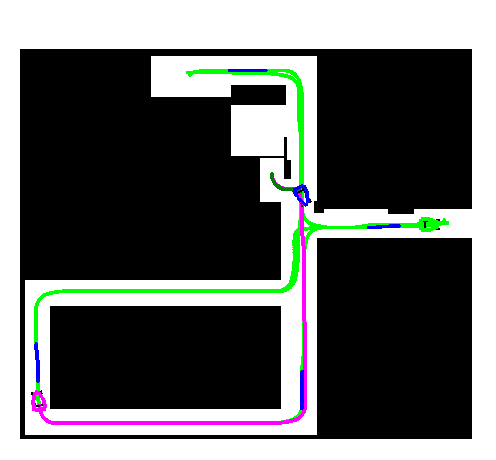
\includegraphics[width=\linewidth]{graphics/AutRnd5_Sim8_path.eps}

%    \caption[`LAGR' timid night watchman.]{A simulation of path induced by an
%      automaton that encodes the behavior patrol the corridors by visiting four
%      specific policy domains is shown.  Upon sensing a `Intruder', the ``timid night
%      watchman'' goes and hides in the corner until the intruder leaves.  Three robots
%      are shown: the initial pose to the right, the final pose when execution is
%      terminated near the middle, and the pose at which the intruder is detected in
%      the lower right.  }
%    \label{fig:lagr_automaton_full_path}
% \end{figure}

% Together, the automaton and policy suite serve as a hybrid control policy.  For these
% specifications, the extracted automaton has 2400 nodes.  Executing the local control
% policies as specified by the automaton induces a continuous system evolution that
% satisfies the high level specification.  At the start of execution, we search the
% entire automaton as a list of nodes until a node is found that has the correct input
% state (Hazard = \FALSE ) and whose associated policy contains the initial pose.  This
% approach, which allows starting from some arbitrary initial pose, works for this
% particular scenario because of the cyclic behavior of the scenario; other scenarios
% might require that the robot start in the domain of a policy in an explicit set of
% initial policies.  A simulation run is shown in \refig{lagr_automaton_full_path}.
% The intruder detector is triggered at an arbitrarily specified time.

% The automaton governs the selection of local control policies.  The automaton
% transitions between nodes as the system pose enters the domain of a policy associated
% with a child node of the current automaton node.  In other words, from node $p_i$, at
% each time step\footnote{The policies are designed as continuous control laws;
%   however, the implementation on a computer induces a discrete time step.  We assume
%   the time step is short compared to the time constant of the closed-loop dynamics.},
% the values of the binary sensor inputs are evaluated. Based on these inputs, all
% valid successor nodes are determined. If the vehicle is in the domain of policy
% $\Phi_{l}$, which is associated with a valid automaton successor node $p_j$, the
% transition is made.  Otherwise, if the vehicle is still in the domain of $\Phi_{k}$,
% which is the active policy associated with node $p_i$, the execution remains in node
% $p_i$.  If a node has more than one child node that represents a valid transition,
% the choice can be made arbitrarily.  For these experiments, the first valid
% transition as defined by the synthesis algorithm is chosen.  This execution based on
% continuous motion is equivalent to the discrete execution of the automaton
% \cite{fainekos_05a,belta_06}.


% \begin{figure}[bt]
%   \centering 
%   \psfrag{2500}{2500}
%   \psfrag{2000}{2000}
%   \psfrag{1500}{1500}
%   \psfrag{1000}{1000}
%   \psfrag{500}{500}
%   \psfrag{Time (s)}{Time (s)}
%   \psfrag{Node ID}{Node ID}
%   \psfrag{Automaton Nodes}{}

%     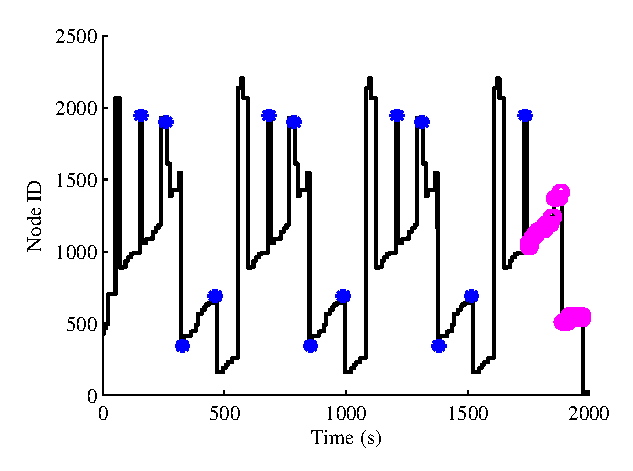
\includegraphics[width=0.7\linewidth]{graphics/AutRnd5_Sim8_nodes.eps}

%     \caption[`LAGR' timid night watch automaton node switching.]{As the system
%       executes, the automaton changes nodes based on the discrete inputs and
%       inclusion of the current pose in a given policy domain.  The graph shows three
%       distinct phases.  The thirteen points marked with '*' indicated the check
%       points passed.  The thickest portion, which is actually closely spaced
%       `$\circ$' symbols, shows the portion where the intruder is detected.  Notice
%       that the system makes multiple passes past each checkpoint before the intruder
%       is detected.}
%    \label{fig:lagr_automaton_full_nodes}
% \end{figure}


% \refig{lagr_automaton_full_nodes} shows the progression of the system through the
% automaton nodes as the system moves through the environment.  Note the cyclic nature
% as the system completes three patrols before the intruder is detected.  As the
% automaton state transitions, so does the associated policy as shown in
% \refig{lagr_automaton_full_policies}.

% \begin{figure}[bt]
%   \centering 
%   \psfrag{3500}{3500}
%   \psfrag{3000}{3000}
%   \psfrag{2500}{2500}
%   \psfrag{2000}{2000}
%   \psfrag{1500}{1500}
%   \psfrag{1000}{1000}
%   \psfrag{500}{500}
%   \psfrag{Time (s)}{Time (s)}
%   \psfrag{Policy ID}{Policy ID}
%   \psfrag{Policy}{}
%    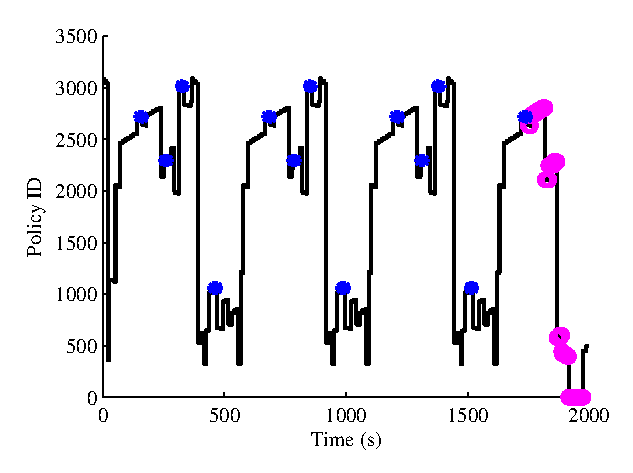
\includegraphics[width=0.7\linewidth]{graphics/AutRnd5_Sim8_policies.eps}

%    \caption[`LAGR' timid night watch policy switching.]{Each node in
%      the automaton is associated with a particular policy in the
%      suite.  As the system executes, the local policies are activated
%      by the automaton based on the local pose estimate.The graph shows
%      the same three distinct phases as
%      \refig{lagr_automaton_full_nodes}.}
%    \label{fig:lagr_automaton_full_policies}
% \end{figure}

% In this execution strategy, the continuous evolution of the system governs the
% discrete transitions in the automaton; therefore, the resultant transitions are
% asynchronous, and not governed by a fixed time step.  In this current implementation,
% the discrete inputs act as guards on the automaton transitions; the discrete input
% must match the value associated with the child node to allow transition into the
% child node, but does not force transition out of the current node.  Another approach
% could check the discrete input at each update step and force transitions out of a
% given automaton node if the inputs do not match the reference input.  This would
% require that each node has a child with the same policy reference, but different
% discrete inputs .

% %%\FloatBarrier

% \begin{figure}[bt]
%   \centering 
%    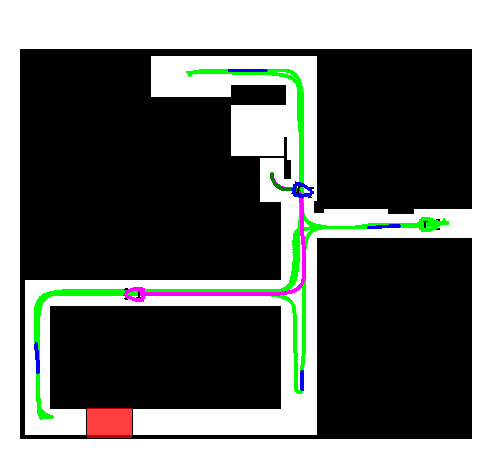
\includegraphics[width=\linewidth]{graphics/AutRnd5_Sim7_path.eps}

%    \caption[`LAGR' timid night watch re-planning.]{As new information
%      becomes available, such the obstacle in the lower corridor, the
%      automaton synthesis formulates a different automaton based on
%      changes to the prepares graph.  The new automaton preserves the
%      correct behavior.}
%    \label{fig:lagr_automaton_blocked}
% \end{figure}


% If the prepares graph changes, the automaton synthesis algorithm must be re-run.
% \refig{lagr_automaton_blocked} shows the simulated path taken when an automaton is
% synthesized for the prepares graph with 24 policies associated with the lower
% corridor invalidated.  The resultant automaton contains 2580 nodes; its execution
% correctly satisfies the original specification by only invoking valid policies.

% %\FloatBarrier

% The automaton synthesis approach guarantees the correct behavior under very
% reasonable assumptions.  First, the automata synthesis only returns an automaton if
% the specification is realizable for the given policy suite and associated prepares
% graph. Second, given a realizable specification, the algorithm is guaranteed to
% produce an automaton such that all its executions satisfy the desired behavior {\bf
%   if} the environment behaves as assumed.  The construction of the automaton is done
% using LTL statements that encode admissible environment behaviors; if the environment
% violates these assumptions, the automaton is no longer correct.  Since the
% specifications encode the transitions allowed by the prepares relationship, the only
% case in which the system pose is not in the domain of $\Phi_{k}$, or in any successor
% $\Phi_{l}$, is if the environment behaved ``badly.''  That is, either some
% disturbance caused the policies to violate the prepares relationship, or the
% environment violated assumptions governing the allowable discrete inputs.  This later
% case requires careful sensor design, with only those restrictions that are
% necessary.  Either case invalidates the automaton.  In the event that a valid
% transition does not exist, the automaton executive raises an error flag, and halts
% the system.  A new plan must be requested.

% Unfortunately, for real systems disturbances are a fact of life.  Policies may be
% designed to be as robust as possible, but disturbances may still take the system out
% of the domain of a currently executing policy.  Often these disturbances are simply
% due to pose estimation updates as described above.  The hybrid control system should
% have a method of recovery, which will likely require some knowledge of the hybrid
% control system and task.  For the task described in this section, our approach is to
% search the automaton as a list of nodes until a node whose associated policy contains
% the current pose estimate and whose discrete input matches the current sensor value;
% as is done for the initial condition. This works in this example because of the
% cyclic nature of the task.  

% A more fundamental problem occurs when the disturbance takes the system outside the
% domain of all policies in the automaton.  Depending on the initial specification, the
% automaton synthesis does not necessarily use every available policy.  As with
% sequence-based approaches, this has a negative impact on the overall robustness of
% the policy composition technique relative to the collection of available policies.
% This thesis considers two approaches to addressing the problem of unused policies.

% The first approach explicitly allows the initial condition to be in any available
% policy and have any allowable sensor value.  The assumption during synthesis that the
% system is in one of two initial policy domains is made to limit the size of the
% automaton.  No assumptions about the initial policies could be made; this would force
% the automaton synthesis to include all policies, but would greatly increase the size
% of the automaton.  The particular implementation of the synthesis algorithm used in
% this thesis precluded this approach; this is not a theoretical issue, later work will
% build a more robust synthesis tool to address this implementation
% issue~\cite{hadas_pc}.

% The second approach, which is used in these experiments, is to augment the
% synthesized automaton to add nodes for each unused policy/sensor combination.  If a
% policy is unused by the original automaton, but prepares another policy that is used
% for all input combinations, then a node is added to the automaton with the unused
% policy as a reference.  This added node ignores the sensor inputs.  The children of
% the added node are all nodes in the automaton whose associated policies are prepared
% by the added node's policy or have the same policy reference.  Since all input
% combinations are covered, a valid child transition will eventually exist.  This
% process is repeated until all policies that prepare others are added to the
% deployment.  This approach maximizes the overall hybrid control policy domain for the
% given collection of domains, while adding the smallest number of nodes to the
% automaton.  This gives the system a way to ``get back on track.''  If the disturbance
% causes the system pose to exit the domains of every policy in the suite, then the
% hybrid control policy will stop the robot and cease execution.  Only by adding
% additional policies, and regenerating the automaton can the system recover.


% \begin{figure}[bt]
%   \centering 
%    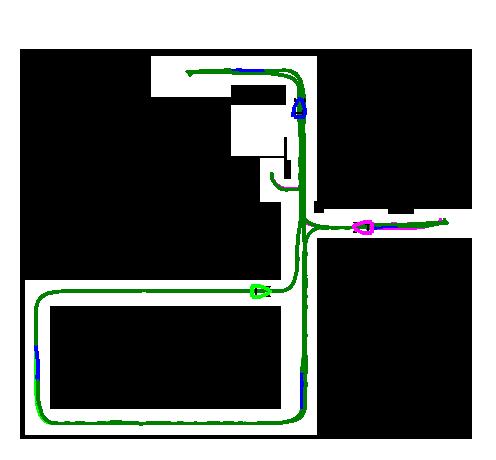
\includegraphics[width=\linewidth]{graphics/AutRnd5_Run4_path.eps}

%    \caption[`LAGR' timid night watch experiments.]{Actual run on
%      LAGR robot.  Here, the robot resumes patrolling after hiding
%      early in the experiment.}
%    \label{fig:lagr_automaton_experiments}
% \end{figure}

% \refig{lagr_automaton_experiments} shows an example run using the augmented
% automaton.  During the experimental runs, the `Intruder' is signaled at will via a
% remote switch.  The experiment successfully satisfies the specification.
% \refig{lagr_automaton_experiments_nodes} shows the progression of nodes during
% execution.  Note that the node ID's above 2400 are those added during the
% augmentation process; without these, the execution would have ceased earlier due to
% disturbances.  Given the augmented automaton, the system is able to search for a node
% whose policy contains the current pose.  Eventually, the execution did quit when a
% disturbance finally took the system out of the domain of all the policies.
% \refig{lagr_automaton_experiments_policies} shows the policy switching induced by the
% augmented automaton.  The experiment was repeated several times; the automaton
% successfully induced the correct behavior each time until disturbances caused the
% system to terminate; this points to the need for more policies to be added to the
% policy suite.

% \begin{figure}[bt]
%   \centering 
%   \psfrag{3500}{3500}
%   \psfrag{3000}{3000}
%   \psfrag{2500}{2500}
%   \psfrag{2000}{2000}
%   \psfrag{1500}{1500}
%   \psfrag{1000}{1000}
%   \psfrag{500}{500}
%   \psfrag{Time (s)}{Time (s)}
%   \psfrag{Node ID}{Node ID}
%   \psfrag{Automaton Nodes}{}
%    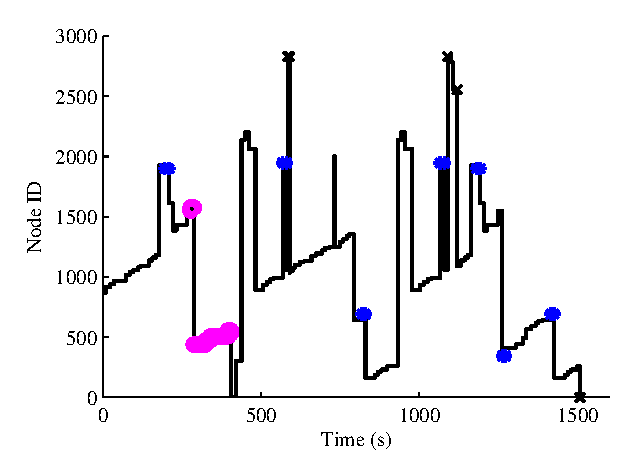
\includegraphics[width=0.7\linewidth]{graphics/AutRnd5_Run4_nodes.eps}

%    \caption[`LAGR' node switching during experiment]{Node switching with
%      invocations of augmented nodes shown by 'x'; the controller would have ceased
%      execution were it not for these added nodes.}
%    \label{fig:lagr_automaton_experiments_nodes}
% \end{figure}



% \begin{figure}[bt]
%   \centering 
%   \psfrag{3500}{3500}
%   \psfrag{3000}{3000}
%   \psfrag{2500}{2500}
%   \psfrag{2000}{2000}
%   \psfrag{1500}{1500}
%   \psfrag{1000}{1000}
%   \psfrag{500}{500}
%   \psfrag{Time (s)}{Time (s)}
%   \psfrag{Policy ID}{Policy ID}
%    \psfrag{Policy}{}
%   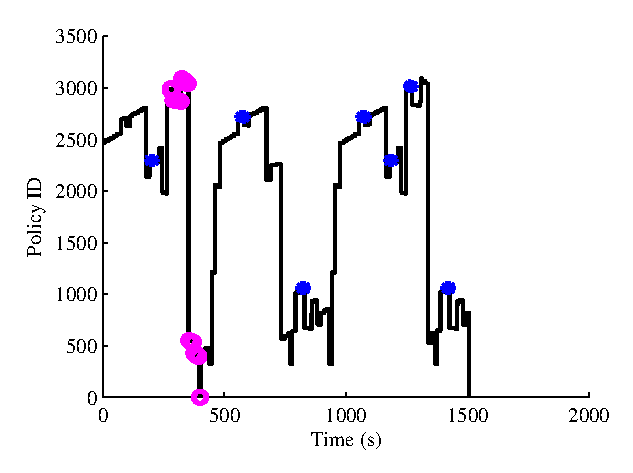
\includegraphics[width=0.7\linewidth]{graphics/AutRnd5_Run4_policies.eps}

%    \caption[`LAGR' policy switching during experiment]{Policy switching during an experiment.}
%    \label{fig:lagr_automaton_experiments_policies}
% \end{figure}

% The drawback to the augment and search approach is that there is no history;
% therefore, the system will sometimes repeat an earlier portion of the patrol loop,
% prior to visiting the other nodes.  This problem could be addressed by adding an
% output that encodes which ``downstream'' check point will be encountered next, and
% using this information to guide the search for a valid node.  This requires
% associating each policy with the closest checkpoint before the synthesis.  One
% possible approach is to choose the checkpoint that generates the least cumulative
% cost for a given policy from a set of costs generated by considering each checkpoint
% as the goal of a policy ordering.  During disturbance recovery, the system searches
% for a node whose associated policy domain contains the current pose and whose
% ``ClosestCheckpoint'' output matches the assigned checkpoint for that policy.

% The automata-base approach is capable of producing complex behaviors, which allow the
% system to react to changes in the environment via the binary environmental inputs.
% Additionally, the automata-based approach allows the system to exhibit desirable
% limit cycles; in this example, repeatedly patrolling a hallway.  Thus automata-based
% approaches are more suitable for repetitive tasks than order-based approaches.  That
% said, the automata should make use of all available policies, and provide a method of
% recovery, in order to maintain robustness to disturbance that is the hallmark of
% order-based approaches.

% %\FloatBarrier%afterpage{\clearpage}

% \subsection{Ackermann Steered Car-like Parking Simulations}
% \label{sec:ackermann_automaton}

% \begin{figure}[bt]%[ht]
% \begin{center}

%  \vspace{0.2in}

%  \includegraphics[width=\linewidth]{graphics/sim_parking_demo.eps} 

%   \caption[Local parking behavior induced by meta-policy]{Parking behavior induced by
%     the composition of local policies.  The feedback control policies guarantee the
%     safety of the maneuver.}
% \label{fig:parking}
% \end{center}
% \end{figure}

% This section provides an example of policy-based planning with the more complex
% system model of an Ackermann steered car.  Here, the scenario is one of searching for
% an available parking space, and then parking.  The environment is known; what is
% unknown is whether a given parking space is available or occupied.  The system has a
% local sensor for detecting open parking spaces; thus, the system must search for an
% available parking space by systematically driving past all the parking spaces.  If an
% open parking space is found, the system changes behavior from searching to parking,
% and executes the parking maneuver as illustrated in \refig{parking}.  The results
% demonstrate coupled planning and control for a complex system that exhibits complex
% behaviors that change based on reactions to the changing environment.

% \begin{figure}[bt]
%   \centering
%   \includegraphics[width=0.7\linewidth]{graphics/sim_parking_run_0_world.eps}
%   \caption[Environment for parking simulations]{The environment has 40 parking spaces
%     arranged around the middle city block.  Initially, there are five empty parking
%     spaces randomly chosen in the environment.}
%   \label{fig:acker_parking_world}
% \end{figure}

% The environment, shown in \refig{acker_parking_world}, consists of two city blocks
% accessible from ten entering roads.  Each road consists of two lanes that follow the
% American standard of driving on the right side.  One block is surrounded by 40
% parking spaces; 20 for the clockwise direction and 20 for the counterclockwise
% direction. The entry/exit points are labeled 1-10 clockwise starting from the
% north/south lanes at the top left of the environment.  The parking spaces are
% identified with a numeric identifier adjacent to each space.  The roadway lanes and
% parking spaces are sized for an urban environment.  The robot system uses an
% Ackermann steered kinematic model that controls the forward velocity and the rate of
% steering angle change; see \reapp{robots} for details.

% \begin{figure}[bt]
%  \begin{center}
%  \begin{minipage}[b]{\linewidth}
%  \begin{minipage}[b]{0.48\linewidth}
%   \centering 
%   \includegraphics[width=\linewidth]{graphics/parkway_details_parking.eps}

%  {\scriptsize a) Policies for parking.}
%    \end{minipage}
%  \hspace{0.03\linewidth} % To get a little bit of space between the figures
%  \begin{minipage}[b]{0.48\linewidth}
%    \centering 
%    \includegraphics[width=\linewidth]{graphics/parkway_details_leaving.eps}

%   {\scriptsize b) Policies for leaving}
%  \end{minipage}

%  \end{minipage}
 
%  \caption[Parking policy details]{Details of policies used for parking
%    and leaving.  The policies, which are shown relative to the cache
%    reference point, are shown wider than normal to show details.  Six
%    policies are associated with parking.  Five policies are used to
%    exit a parking space and prepare policy in the traffic lane.}
%   \label{fig:parkway_details}
% \end{center}
% \end{figure}

% The parking demonstrations use a collection of 16 \PF style policies, which are
% instantiated in the policy cache relative to the origin.  The cache includes policies
% for traveling straight down a roadway lane, for parking and leaving a given space,
% and for turning at intersections.  \refig{parkway_details} shows examples of the
% policies for parking and leaving, which treated as meta-policies for planning
% purposes.  Associated with the inlet policy of the parking policy is a sensor that
% determines whether the parking space is available.  If the parking space is
% unavailable, then the parking meta-policy prepares some other policy further down the
% roadway lane.  \refig{parkway_intersection} shows an example intersection, the
% deployed policies, and the extent of the robot body into the workspace.  Since this
% is a simulation, only those policies needed for basic traffic are deployed.  No
% attempt is made to fill the free pose space in order to provide robustness.


% \begin{figure}[bt]
%  \begin{center}
%  \begin{minipage}[b]{\linewidth}
%  \begin{minipage}[b]{0.48\linewidth}
%   \centering 
%   \includegraphics[width=\linewidth]{graphics/parkway_intersection_lanes.eps}

%   \end{minipage}
%  \hspace{0.03\linewidth} % To get a little bit of space between the figures
%  \begin{minipage}[b]{0.48\linewidth}
%    \centering 
%    \includegraphics[width=\linewidth]{graphics/parkway_intersection_padded.eps}

%  \end{minipage}

%  \begin{minipage}[b]{0.48\linewidth}
%   \centering 

%   {\scriptsize a) Connected policy domains projected into workspace}

%  \end{minipage}
%  \hspace{0.03\linewidth} % To get a little bit of space between the figures
%  \begin{minipage}[b]{0.48\linewidth}
%    \centering 

%    {\scriptsize b) Body extent over the policy domains}

%  \end{minipage}
%  \end{minipage}
 
%  \caption[Policies deployed at intersection]{Deployment of policies at an
%    intersection.  The polices include those that pass straight through the
%    intersection, as well as left and right turns.  Other policies are used to tie the
%    straight sections to the turns.  The policy domains, which are widened to increase
%    visibility, appear as thick lines in (a).  }
%   \label{fig:parkway_intersection}
% \end{center}
% \end{figure}

% For the simulations in this section, a total of 306 policies are deployed in the
% environment.  The regularity of the environment allows an automated approach to
% policy instantiation based on a collection of reference points defined relative to
% the intersections and parking spaces.  The policy total includes 40 parking
% meta-policies and 40 leaving meta-policies, as well as 24 each left, right and
% straight maneuvers at the six intersections.  Policies to enter and leave the
% environment are added at the 10 roadways connecting the environment to the outside
% world.  Given the suite of 306 policies, the prepares graph is automatically defined
% as described in \resec{nonholo}.


% %\FloatBarrier%afterpage{\clearpage}

% \subsubsection{Basic Parking Scenarios}
% \label{sec:acker_parking}

% The basic scenario considers a single car that must park in the environment.  The
% environmental input is a sensor called `\PARK' that tells the car if a parking space
% is available; the system output identifies which policy to activate.  The car may
% enter from any of the ten roadways connecting to the two blocks.  The car can only
% determine whether there is a free parking space if we are in a policy next to it.
% This means that `Park' cannot become \TRUE\ if the vehicle is not next to a parking
% space or in one. Also, for implementation reasons, we assume that the input `Park'
% remains \TRUE\ after parking.  We have no assumptions on the goals of the environment,
% and make no assumptions about the availability of an empty parking spot.  The
% allowable system transitions include the transitions of the prepares graph, the
% vehicle cannot park if there is no parking space available, as indicated by the
% `Park' input, and if there is an empty parking space the car must park; removing the
% last restriction may allow the vehicle to pass an open spot before parking.  The
% system goal encodes a list of policies the vehicle must visit infinitely often if it
% has not parked yet.  The list of policies to visit defines the area in which the
% vehicle will look for an available parking space; in this case, the visit policies
% correspond to the eight lanes around the parking spaces (four going clockwise and
% four going counter clockwise).  Note, this goal condition is true if either the
% vehicle visits these policies infinitely often (when there is no parking space
% available) or it has parked.  Defining a different list of policies to visit would
% change the search strategy induced by the automaton.  Additional specifications could
% be written to tie the search strategy to the point of entry, but this would increase
% the size and complexity of the automaton.

% For simulations shown in Figures~\ref{fig:acker_parking_runs_12}
% and~\ref{fig:acker_basicSim}, a new vehicle is introduced at a random entrance.  The
% parking spaces are filled according to the previous run.  As the automaton executes,
% if a parking policy is a successor to the current state, the empty/occupied status is
% checked via the local `Park' sensor. This work does not address the required sensor,
% but assumes a binary output.  Transition to the parking policy is enabled if the
% associated space is empty.  If the transition is enabled, `Park' remains \TRUE\ so that
% other transitions are disabled until the vehicle pose enters the domain of the
% parking meta-policy, and the system parks.  Six runs are simulated using the global
% parking automaton; The first five runs park.  In Run \#6, there are no parking spaces
% available; therefore, the vehicle continues to circle past every possible parking
% space, waiting on another vehicle to leave.



%  \begin{figure}%[tb]
%    \begin{center}
%    \begin{minipage}[b]{\linewidth}
%    \begin{minipage}[b]{0.44\linewidth} 
%    \centering 
%    \includegraphics[width=\linewidth]{graphics/sim_parking_run_1_world.eps}   
  
%    \vspace{-1.6ex}
%    {\small Run \#1} 
%    \end{minipage}
%   \hspace{0.03\linewidth}
%   \begin{minipage}[b]{0.44\linewidth}
%    \centering  
%    \includegraphics[width=\linewidth]{graphics/sim_parking_run_2_world.eps} 
  
%    \vspace{-1.6ex}
%    {\small Run \#2}
%  \end{minipage} 
%  \end{minipage}  
%  \caption[Two executions of parking simulation]{Two executions of the basic parking
%    scenario.  The initial conditions for each run are circled. }
%     \label{fig:acker_parking_runs_12}

%  \end{center}
%  \end{figure}

%  \begin{figure}%[tb]
%    \begin{center}
%    \begin{minipage}[b]{0.44\linewidth} 
%    \centering 
%    \includegraphics[width=\linewidth]{graphics/sim_parking_run_3_world.eps}   
  
%    \vspace{-1.6ex}
%    {\small Run \#3} 
%    \end{minipage}
%   \hspace{0.03\linewidth}
%   \begin{minipage}[b]{0.445\linewidth}
%    \centering  
%    \includegraphics[width=\linewidth]{graphics/sim_parking_run_4_world.eps} 
  
%    \vspace{-1.6ex}
%    {\small Run \#4}
%  \end{minipage} 

%    \vspace{0.5ex}

%    \begin{minipage}[b]{0.44\linewidth} 
%    \centering 
%    \includegraphics[width=\linewidth]{graphics/sim_parking_run_5_world.eps}   
  
%    \vspace{-1.6ex}
%    {\small Run \#5} 

%    \end{minipage}
%   \hspace{0.03\linewidth}
%   \begin{minipage}[b]{0.44\linewidth}
%    \centering  
%    \includegraphics[width=\linewidth]{graphics/sim_looping_run_6_world.eps}
 
%    \vspace{-1.6ex}
%    {\small Run \#6}

%  \end{minipage} 

 
%  \caption[Four executions of parking simulation]{Four executions of the basic parking
%    scenario.  The initial conditions for each run are circled.  The last run
%    continues to loop as no parking spaces are available. }
%     \label{fig:acker_basicSim}

%  \end{center}
%  \end{figure}

% %%\FloatBarrier
% %
% % \subsection{Multi-vehicle Scenarios}
% % \label{sec:acker_multi_car}
% %
% % The automata-based approach to policy composition naturally extends to multi-agent
% % systems~\cite{hadas_07}.  The local policies guarantee predictable local behavior of
% % a single agent; the automata governs the switching between local policies to
% % coordinate the high-level behavior of an agent.  Taking this approach further,
% % Kress-Gazit \ea~\cite{hadas_07} use the environmental inputs to coordinate behavior
% % between agents using automata.  Each agent runs its own automata-based hybrid
% % controller, which responds to other agents via environmental inputs; that is, the
% % outputs of one agent become inputs to another agent.  This section details a
% % simulation using the policy composition approach advocated in this thesis with the
% % automata-based multi-agent coordination scheme advocated in~\cite{hadas_07}.  The
% % simulation results illustrate several issues that arise with this approach.
% %
% % In order to expand the basic parking approach to allow for multiple vehicle
% % scenarios, the LTL formulas from above are modified.  The approach uses an additional
% % input and several outputs.  The additional input is `Hazard', which causes the
% % vehicle to stop in place.  The hazard can be triggered by proximity to another
% % vehicle, or by an external device such as a stop-light.  When the hazard clears, the
% % robot should resume motion as before.  In a real system, many hazards can be avoided
% % by slowing down, and waiting for the other vehicle to clear.  For simplicity, these
% % simulations require the system to stop.  When the vehicle stops in response to a
% % `Hazard', the system outputs `\STOP'.  Additional outputs signal `\LEFT' and `\RIGHT'
% % as appropriate.  There are also outputs that signal the vehicles intentions for
% % `Parking' and `Leaving'.  The automaton outputs can be sensed by other vehicles in
% % the environment.

% % The LTL specifications from above are modified to take the new inputs
% % and outputs into consideration, and allow a new ``leaving'' behavior.
% % Each vehicle in the simulation runs a local copy of one of two
% % automata.  The only coordination is via the individual `Hazard'
% % sensor.  We now consider each automaton in turn.

% % \paragraph{Parking Automaton}
% % The parking automaton for the multi-vehicle scenario is similar to the individual
% % case, but includes the stopping behavior and the additional outputs.  The system
% % transitions include all the conditions of the individual parking case, plus the
% % conditions that activate the outputs for turning, stopping, or parking as needed.
% % The system goal is includes the parking conditions, but also allows for a vehicle to
% % remain stopped if a broken stop-light or accident ahead blocks the roadway.  With
% % these specifications, the parking automaton has 2142 nodes.


% % \paragraph{Leaving Automaton}
% % In this scenario, a vehicle is leaving its parking space and exiting the block via
% % some specified exit. The leaving automaton for the multi-vehicle scenario has an
% % extra input that specifies which of the ten possible exits the vehicle will exit.
% % The initial environment specification is such that only one exit is specified.  Two
% % different vehicles leaving two different parking spots may use the same synthesized
% % automaton with different inputs that designate the desired exit.  We require the exit
% % specification to be constant, meaning it cannot change once it is given.  We make no
% % assumptions on the infinite behavior of the environment, therefore the goal component
% % remains set to \TRUE.  Initially, the car is leaving a parking space, hence it must
% % turn on the left turn signal.

% % The system transitions are include the policy prepares relations, which policies turn
% % on the left/right signals, and always stop on hazard.  The system goal specifies that
% % the vehicle must go to the designated exit policy unless it stops.  With these
% % specifications the leaving automaton has 1908 nodes.

% % The key to using these automata in a decentralized multi-agent scenario is the
% % coordination provided by the `Hazard' sensor.  Each vehicle executes its own hazard
% % sensor with a single binary value `Hazard.'  The `Hazard' input is based on either a
% % timed stop-light or a proximity/precedence sensor.  The stop-light alternates between
% % north/south and east/west travel along the roadways.  Each intersection transitions
% % at the same time; there is a slight overlap where all directions are stopped.  Any
% % vehicle entering the policies just before the left/right/straight policies at each
% % intersection checks the current value of the stop-light.  If the ``red light'' is
% % visible, the `Hazard' flag is set to \TRUE.

% % The `Hazard' sensor is a discrete hybrid automaton in its own right, that attempts to
% % determine precedence based on the robot's internal state and binary outputs, and the
% % other robots relative pose, velocity, and binary outputs.  Thus the ``sensor'' is a
% % mixture of continuous measurements and discrete logic.  The `Hazard' checks proximity
% % of other vehicles, and determines the precedence relationships between vehicles; that
% % is, which vehicle must yield to the other.  For this simulation, the `Hazard' sensor
% % is hand-coded and tuned to given the proper performance.  The sensor automaton sets
% % `Hazard' to \TRUE\ whenever the car is too close to a car ahead of it (keeping safe
% % distance), whenever a car ahead is backing up to park (being polite), whenever the
% % car is leaving a parking space and another car passes by and whenever another car is
% % leaving a parking space which the car will park in next.  In this decentralized
% % coordination scheme, each vehicle's `Hazard' sensor must infer the intentions of the
% % others based their outputs.  There is no centralized communication of intentions.

% % \begin{figure}[bt]%[tb]
% %   \begin{center}
% %   \begin{minipage}[b]{0.45\linewidth} 
% %   \centering 
% %   \includegraphics[width=0.9\linewidth]{graphics/sim_hazard_run_7a.eps} 
  
% %   {\small Run \#7 - a} 

% %   \end{minipage}
% %  \hspace{0.03\linewidth}
% %  \begin{minipage}[b]{0.45\linewidth}
% %   \centering  
% %   \includegraphics[width=0.9\linewidth]{graphics/sim_hazard_run_7b.eps} 

% %   {\small Run \#7 - b}
% % \end{minipage} 

% % \caption[Simple multi-vehicle traffic simulation]{In this continuation of Run \#6,
% %   the two snap shots show a simple multiple vehicle scenario.  A timed stop-light
% %   triggers a `hazard' input that causes the vehicle heading east to stop.  This
% %   allows the vehicle from Run\#6 to travel through the intersection, and eventually
% %   park in the newly available parking spot.}
% %    \label{fig:acker_multipleSim}

% % \end{center}
% % \end{figure}

% % \refig{acker_multipleSim} shows the continuation of Run \#6 with the
% % hazard inputs added to the parking automaton, and the new leaving
% % automaton controlling the second vehicle.  In the first snapshot,
% % vehicle \#6 is just beginning to approach the intersection, while
% % vehicle \#7 stops for the light.  The second snapshot shows vehicle
% % \#7 dutifully waiting for the signal, while vehicle \#6 has passed
% % through the intersection.  Although not shown, after the stop-light
% % changes, vehicle \#7 exits the area and vehicle \#6 continues around
% % under the control of the global parking automaton and parks in the
% % newly open spot.

% % %%\FloatBarrier

% % \begin{figure}[bt]
% %   \centering
% %   \includegraphics[width=0.60\linewidth]{graphics/sim_parking_run_5_t1591.eps}
% %   \caption[Snapshot of complex multi-vehicle traffic simulation]{A snapshot of a more
% %     complex multi-vehicle simulation.  Each vehicle executes an
% %     automaton that encodes the high-level specification ``stop on
% %     hazard'' and either ``drive around until you find a free parking
% %     space and then park'' or ``leave your parking space and exit the
% %     block''.  Coordination between robots is done via an individual
% %     `Hazard' sensor in a decentralized approach.  This snapshot is
% %     taken at 15.91 seconds.}
% %   \label{fig:acker_multi_run1}
% % \end{figure}

% % \refig{acker_multi_run1} shows an example of a more complex multi-vehicle simulation.
% % At this point in time, seven cars are moving in the workspace.  Initially, 35 of the
% % 40 parking spaces were randomly specified as occupied.  In this simulation, eight
% % cars enter the block at different times and from different entry points, looking for
% % a parking space. The times and entry points are (t=0.06 seconds, Entry = 10),
% % (1.0,2), (2.0,7), (5.0,8), (7.0, 5), (10.0,6), (15.0, 8), (22.0,5).  During the
% % execution, three cars leave their parking spaces and exit the workspace.  The times,
% % parking spaces, and exit point are (t=13.0, Parking=23,exit=1), (15.0, 6, 7), and
% % (30.0, 32, 5).  The simulation runs until 76.33 seconds of elapsed time when the last
% % car exits or is parked.  \refig{simGeneral} shows a general snapshot of the
% % simulation at a later time.  Cars whose `Stop' output is \TRUE\ are marked with red
% % ellipses; that is, those cars who stop because the `Hazard' input is \TRUE.  The
% % three stopped cars in \refig{simGeneral} are obeying stop-lights.

% % \begin{figure}[bt]
% %   \centering
% %   \includegraphics[width=0.6\linewidth]{graphics/sim_parking_run_5_t3133_Haz.eps}
% %   \caption[Later snapshot of multi-vehicle simulation]{A later
% %     snapshot taken at 31.33 seconds during the simulation. In this
% %     figure, cars surrounded by red ellipses are cars that are stopping
% %     due to the `Hazard' input signaled by the timed stop-light.}
% %   \label{fig:simGeneral}
% % \end{figure}

% % %%\FloatBarrier

% %  \begin{figure}[bt]
% %    \begin{center}
% %    \begin{minipage}[b]{\linewidth} 
% %    \begin{minipage}[b]{0.45\linewidth} 
% %    \centering 
% %    \includegraphics[width=\linewidth]{graphics/sim_parking_run_5_t1591_Haz_close.eps}   
% % %  
% %    \vspace{0.4ex}
% %    {\small (a) Blue car leaving (t=15.91 s)} 
% %    \end{minipage}
% %   \hspace{0.03\linewidth}
% %    \begin{minipage}[b]{0.431\linewidth} 
% %    \centering 
% %    \includegraphics[width=\linewidth]{graphics/sim_parking_run_5_t3469_Haz_close.eps}   
% % %  
% %    \vspace{0.4ex}
% %    {\small (b) Red car parking (t=34.69 s)} 
% % %
% %    \end{minipage}
% %    \end{minipage}
% %  %

% %    \vspace{0.8ex}

% %    \begin{minipage}[b]{\linewidth} 
% %    \begin{minipage}[b]{0.46\linewidth}
% %    \centering  
% %    \includegraphics[width=\linewidth]{graphics/sim_parking_run_5_t1629_Haz_close.eps} 
% % %
% %    \vspace{0.4ex}
% %    {\small (c) Yielding to turn in progress (t=16.29s)}
% %  \end{minipage} 
% %   \hspace{0.03\linewidth}
% %    \begin{minipage}[b]{0.45\linewidth} 
% %    \centering 
% %    \includegraphics[width=\linewidth]{graphics/sim_parking_run_5_t2641_Haz_close.eps}   
% % %  
% %    \vspace{0.4ex}
% %    {\small (d) Two cars parking (t=26.41s)} 
% % %
% %    \end{minipage}
% %    \end{minipage}
% % %
% %   \vspace{0.8ex}
% % %
% % %  
% %     \begin{minipage}[b]{\linewidth} 
% %  \begin{minipage}[b]{0.45\linewidth}
% %    \centering  
% %    \includegraphics[width=\linewidth]{graphics/sim_parking_run_5_t2718_Haz_close.eps}
% % % 
% %    \vspace{0.4ex}
% %    {\small (e) Two cars parking (t=27.18)}
% % %

% %  \end{minipage} 
% %   \hspace{0.03\linewidth}
% %   \begin{minipage}[b]{0.45\linewidth}
% %    \centering  
% %    \includegraphics[width=\linewidth]{graphics/sim_parking_run_5_t4639_Haz_close.eps}
% % % 
% %    \vspace{0.4ex}
% %    {\small (f) Two cars at stop-light (t=46.39s)}
% % %
% %  \end{minipage} 
% %  \end{minipage} 
% % %
 
% %  \caption[Close up of multi-vehicle behaviors]{Close up looks at different behaviors
% %    seen throughout the simulation.  }
% %     \label{fig:aker_multi_SimClose}
% % %
% %  \end{center}
% %  \end{figure}

% %  \refig{aker_multi_SimClose} shows several close up looks at different traffic
% %  behaviors encountered during the simulation. In (a), the blue car which is leaving
% %  the parking space has stopped, indicated by a red ellipse, to let the brown car
% %  drive by. This `Hazard' was invoked based on a ``proximity sensor.'' In (b), red car
% %  is parking while the blue car waits for it to finish before passing.  In (c), the
% %  orange car is stopping to allow the gray car to complete a left turn, according to
% %  the precedence established by the individual car's `Hazard' sensors.  The white car
% %  on the left is leaving the parking space that later will be occupied by the brown
% %  car. Figures~\ref{fig:aker_multi_SimClose}-d and (e) are two snapshots of two cars
% %  parking simultaneously in opposite lanes. The car that started the parking maneuver
% %  later (bottom lane) pauses to allow the other car to park safely.
% %  \refig{aker_multi_SimClose}-f shows two cars stopping before a stop-light. While the
% %  white car stopped based on the stop-light, the black car behind stopped based on the
% %  proximity to the car ahead of it.

% % %\FloatBarrier

% %  Sensors, or more specifically the binary inputs used by the automaton, are
% %  fundamental to the success of this decentralized approach.  First, as mentioned
% %  above, the sensors must satisfy the assumptions made about them in the LTL formulas
% %  for the environment; otherwise the automaton will not be correct. Failing to trigger
% %  `Hazard' may allow collision as the local policies do not consider obstacle
% %  avoidance.  Second, even if the sensors do satisfy these assumptions, they may still
% %  cause correct, yet unintended behavior. For example, if the proximity sensor set the
% %  `Hazard' input to \TRUE\ whenever another vehicle was in a certain radius, even if the
% %  other vehicle was behind in a forward driving lane, both vehicles may get
% %  deadlocked; that is, both would stop forever.  While this behavior satisfies the
% %  original specification, it does not follow the spirit of finding a parking space.
% %  On the other hand, both cars stopping might be a desired behavior when an accident
% %  occurred, therefore we would not want to forbid it in the specifications.
 
% %  Currently, there are no guarantees that the implemented `Hazard' sensor automaton is
% %  correct in all cases, and will not introduce deadlock.  Such unintended behavior
% %  would not be present in a centralized approach where the controller has full
% %  knowledge and not just local information as is the case here; however, the
% %  centralized approach does not scale well.  The decentralized approach, which does
% %  scale well for additional robots, may deadlock for a poorly designed hazard sensor;
% %  thus, much work remains to develop automatic ways of specifying the `Hazard' sensor
% %  automaton and prove that the composition of these multiple automata is free of
% %  deadlock.
% %  %This is a classical problem in concurrent systems; fairness
% %  %assumptions must be imposed on the inputs to ensure that the system
% %  %will not deadlock.

% % %\FloatBarrier

% \subsection{Summary}
% \label{sec:planning_summary}

% This chapter has presented several experiments which validate the approach advocated
% in this thesis.  The approaches to planning in the space of control policies, and
% composing local policies to induce the desired behavior, is demonstrated with
% experiments on real robots and simulations on realistic systems.  A range of planning
% approaches and scenarios are demonstrated.  To our knowledge, this is the first
% experimental verification of these techniques on real wheeled mobile robots with
% non-circular body shapes; that is, body shapes where orientation is fundamental to
% the safety of the approach.

% Several broad conclusions can be drawn from these results.  In general, order-based
% approaches are preferred over sequence based approaches due to the enlarged domain;
% this is in keeping with the aim of designing ``global'' policies.  Automata-based
% approaches are useful for generating complex reactive tasks; the policy composition
% approach advocated in this thesis extends these techniques to real world, complex
% systems.

% Overall, the results validate the approach; however, several issues have been
% identified.  First, the policies can only induce behaviors that the system execute.
% If the mechanical system is incapable responding to the controls, the properties of
% composable policies will be violated.  Thus, either the system dynamics must be
% modified, the policies redesigned, or additional policies added to provide more
% robustness.  Since disturbances are a fact of life, automata-based approaches should
% make use of all available policies in keeping with the global policy theme, and
% provide a method of recovery in the face of large disturbances.  The hybrid control
% policy should also have a method of identifying undesirable limit cycles, and have a
% recovery strategy.  Finally, while the automata-based approach to decentralized
% multi-agent control is promising, the design of a hybrid sensor automata, which can
% provide provably correct performance with the composition of individual automata,
% remains an open problem.






\section{Automata Based Planning}
\label{sec:planning_detailed}

%Automata are more flexible than sequence-based approaches because they
%allow the hybrid control system to react to changes in the environment
%encountered during run time.  
{\large not talking about sequence approachs in this paper, but ideas
  this paragraph might be useful in intro} Like sequence-based
approaches, automata-based switching strategies are capable of
addressing multiple tasks; however, automata have the added advantage
of changing behaviors during runtime based on gathered information
without requiring re-planning.  Combining the policy composition
approach advocated in this thesis with automaton synthesis tools such
as those of~\cite{hadas_07} enables a constructive approach to
building a hybrid control policy whose continuous execution satisfies
high level specifications, while enabling the constrained system to
react to environmental changes.

{\large move idea here into the approach section }
This section presents several experiments and simulations using the synthesis
approach given in~\cite{hadas_07}.  As discussed in \resec{fully}, \cite{hadas_07}
uses a disjoint workspace decomposition and adjacency graph to choose policies based
on our fully actuated policies for idealized systems.  In contrast, this section
defines the specifications and automata synthesis in terms of the prepares graph.
This approach is more flexible because it can be applied to constrained systems, and
allows for overlapping policy domains.


The first example is termed the ``timid night watchman.''  The LAGR robot is tasked
with patrolling office corridors by visiting four checkpoints in turn.  If an
intruder is detected, as indicated by a binary sensor called `Intruder', the robot is
to ``run and hide'' in the small nook near the workspace center; after the intruder
is gone, the robot should resume patrolling.  The system also includes a `Hazard'
input; upon sensing a hazard, the robot should stop in place.  The robot resumes
motion when the hazard is clear.  The robot has three outputs: `Stop', which
indicates that the robot should cease executing its local policy and stop in place,
`CheckPoint', which means the robot is at a designated checkpoint, and $\CP_i$, which
encodes which policy is associated with the automaton node\footnote{Technically, this
  policy ID is encoded as a collection of binary outputs that encode the numeric
  identifier.  For clarity, we will use a simple binary proposition based on the
  numeric identifier for each policy.}.  $\CP_i$ is a binary proposition that is true
when the current state is in the domain of policy $i$.

The behavior is encoded in linear temporal logic (LTL) and input to the automaton
synthesis algorithm as $\varphi=\prl{\varphi_e \Rightarrow \varphi_s}$.  The LTL
formula $\varphi_e$ is an assumption about the inputs, and thus about the behavior of
the environment; the $\varphi_s$ formula represents the desired behavior of the
system.  More specifically,
\[
\bba{ccl}
\varphi_e & = & \varphi_i^e \wedge \varphi_t^e \wedge \varphi_g^e\,, \nonumber\\
\varphi_s & = &\varphi_i^s \wedge \varphi_t^s \wedge \varphi_g^s\,.\nonumber
\eba
\]
The formulas $\varphi_i^e$ and $\varphi_i^s$ describe the initial condition of the
environment and the system. $\varphi_t^e$ represents the assumptions on the
environment by constraining the next possible input values based on the current input
and output values. $\varphi_t^s$ constrains the transitions the system can make,
including obeying the prepares graph.  $\varphi_g^e$ and $\varphi_g^s$ represent the
assumed goals of the environment and the desired goals of the system, respectively.
% For a detailed description of these formulas the reader is referred to \cite{icra_07}.

The automaton synthesis algorithm used by~\cite{hadas_07} takes the initial
conditions, transition relations, and goals, then checks whether the specification is
realizable.  If it is, the algorithm extracts a possible, but not necessarily unique,
automaton that implements a strategy that the system should follow in order to
satisfy the desired behavior.  The automaton synthesis is viewed as a game played
between the environment, which controls the inputs, and the robot which controls the
outputs.  The two players have initial conditions defined by $\varphi_i^e$ and
$\varphi_i^s$.  The way the game is played is that at each step, first the
environment makes a transition according to $\varphi_t^e$, and then the system makes
its own transition according to $\varphi_t^s$.  If the environment can falsify
$\sigma = \prl{\varphi_g^e\Rightarrow\varphi_g^s}$ regardless of the system
transition, we say that the environment is winning and the desired behavior is
unrealizable; this means that there is no automaton that can satisfy the
requirements.  However, if the system can satisfy the desired behavior encoded by
$\sigma$, no matter what the environment does, we say that the system is winning and
we can extract an automaton.

Note that there are two ``ways'' for the system to win. It wins if
either $\varphi_g^s$ is satisfied, i.e.  the system reaches its goals,
\textbf{or} $\varphi_g^e$ is falsified.  The later case implies that
if the environment does not satisfy its goals (either a faulty
environment or the system interfered), then a correct behavior of the
system is no longer guaranteed.  Furthermore, if during an execution
of the automaton the environment violates its own transition relation
encoded by $\varphi_t^s$, the automaton is no longer valid.  The
implication of this is discussed below.

Using the specific ``timid night watchman'' task, the behaviors are encoded as
follows.  The environmental inputs are `Hazard' and `Intruder'.  The system outputs
are those that specify which policy to activate, the `Stop' command, and the
`CheckPoint' flag.  The Hazard input is initially clear, so $\varphi_i^e =
\NOT\mrm{Hazard}$.  There are no other assumptions about the environment;
therefore,$\varphi_t^e = \ALWAYS\TRUE$ and $\varphi_g^s = \ALWAYS\EVENTUALLY\TRUE$.
That is `Intruder' input can have any initial value, and the inputs can change at
will, with no final goal.  The system state is assumed to be in one of two initial
policy domains, the initial policies are not checkpoints, and the system is not
stopped by hazard; therefore,
\[\varphi_i^s = \prl{\CP_1
  \OR\CP_3}\,\AND\,\NOT\STOP\,\AND\,\NOT\mrm{CheckPoint}\,.\] 
The system transitions include knowledge of the prepares graph; thus, using the same
prepares graph as \resec{lagr_total_order}, define
\[\varphi_\Gamma^s = \bigwedge_i \;\Box(\Phi_i\;\Rightarrow\;\prl{\bigcirc
  \Phi_i\bigvee_{j\in \mrm{SuccessorsOfPolicy}_i}\bigcirc \Phi_j}\,.
\] In English, ``it is always true that if the current state is in $\Do{\Phi_i}$ this
time step, the next step will find the state in either $\Do{\CP_i}$ or one of its
successors.''  The set of successors is defined by the prepares graph.  The system
stops if and only if there is a hazard sensed; that is $\varphi_\mrm{haz}^s =
\prl{\NEXT\mrm{Hazard}\IFF\NEXT\STOP}$~\footnote{The ``if and only if'', denoted
  $\IFF$, is a binary proposition that is true if both sides have the same truth
  value, and false otherwise.  Thus, $\prl{\FALSE\IFF\FALSE}$ is true.}.  The system
also encodes that the policy reference does not change if the system stops; that is,
\[\varphi_\mrm{stop}^s = \ALWAYS\prl{\prl{\NEXT\mrm{Hazard}
    \OR\STOP}\,\AND\,\CP_i} \Rightarrow \NEXT\CP_i\,.\] If an intruder is
sensed, and the system is hidden in the nook, the system should stay in the nook;
that is
\[\varphi_\mrm{hide}^s =
\ALWAYS\prl{\NEXT\mrm{Intruder}\,\AND\,\CP_1}\Rightarrow\NEXT\CP_1\,,\]
where $\CP_1$ is the policy that stops the system in the nook.  The system should
resume patrol if the intruder is not sensed; that is
\[\varphi_\mrm{unhide}^s =
\ALWAYS\prl{\NOT\NEXT\mrm{Intruder}\,\AND\,\NOT\mrm{Hazard}\,\AND\,\NOT\STOP}\Rightarrow\NOT\NEXT\CP_1\,.\]
If the robot is at a checkpoint, the CheckPoint output is set; that is
\[\varphi_\mrm{chk}^s=\ALWAYS\prl{\prl{\NEXT\CP_{70}}\,\OR\, \prl{\NEXT\CP_{258}}\,\OR\, \prl{\NEXT\CP_{200}}\,\OR\,
  \prl{\NEXT\CP_{291}}\,\IFF\,\NEXT\mrm{CheckPoint}}\,,\] where 70, 258, 200, and 291
denote the policy domains assigned as checkpoints.  Together, the system transitions
are encoded as
\[\varphi_t^s = \varphi_\Gamma^s\,\AND\,\varphi_\mrm{haz}^s\,\AND\,
\varphi_\mrm{stop}^s\,\AND\,\varphi_\mrm{hide}^s\,\AND\,\varphi_\mrm{unhide}^s\,\AND\,\varphi_\mrm{chk}^s\,.\]
The desired behavior, given as the system goal, is
\[\varphi_g^s=\left\{
\bba{c}
\ALWAYS\EVENTUALLY\prl{\CP_{70}\,\OR\,\mrm{Intruder}\,\OR\,\STOP}\,\AND\\
\ALWAYS\EVENTUALLY\prl{\CP_{258}\,\OR\,\mrm{Intruder}\,\OR\,\STOP}\,\AND\\
\ALWAYS\EVENTUALLY\prl{\CP_{200}\,\OR\,\mrm{Intruder}\,\OR\,\STOP}\,\AND\\
\ALWAYS\EVENTUALLY\prl{\CP_{291}\,\OR\,\mrm{Intruder}\,\OR\,\STOP}\,\AND\\
\ALWAYS\EVENTUALLY\prl{\CP_1\,\OR\,\NOT\mrm{Intruder}\,\OR\,\STOP}
\eba
\right.
\,.
\]
The automaton synthesis satisfies the goals in order.  Therefore, as long as the
intruder is not seen, the automaton implicitly encodes go from 70, to 258, to 200,
and finally to 291 before repeating the cycle. 
 
\begin{figure}[bt]
  \centering 
   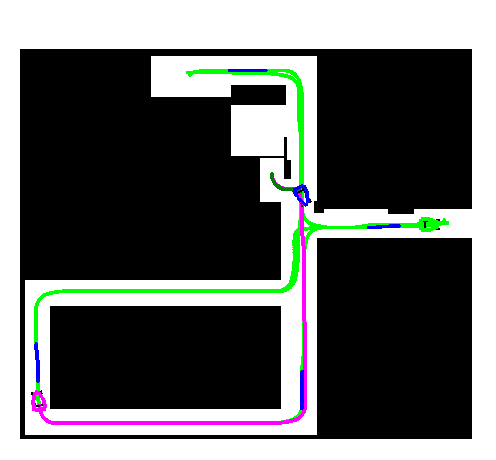
\includegraphics[width=3in]{graphics/AutRnd5_Sim8_path.eps}

   \caption[`LAGR' timid night watchman.]{A simulation of path induced by an
     automaton that encodes the behavior patrol the corridors by visiting four
     specific policy domains is shown.  Upon sensing a `Intruder', the ``timid night
     watchman'' goes and hides in the corner until the intruder leaves.  Three robots
     are shown: the initial pose to the right, the final pose when execution is
     terminated near the middle, and the pose at which the intruder is detected in
     the lower right.  }
   \label{fig:lagr_Aautomaton_full_path}
\end{figure}

Together, the automaton and policy suite serve as a hybrid control policy.  For these
specifications, the extracted automaton has 2400 nodes.  Executing the local control
policies as specified by the automaton induces a continuous system evolution that
satisfies the high level specification.  At the start of execution, we search the
entire automaton as a list of nodes until a node is found that has the correct input
state (Intruder = false) and whose associated policy contains the initial pose.  This
approach, which allows starting from some arbitrary initial pose, works for this
particular scenario because of the cyclic behavior of the scenario; other scenarios
might require that the robot start in the domain of a policy in an explicit set of
initial policies.  A simulation run is shown in \refig{lagr_Aautomaton_full_path}.
The intruder detector is triggered at an arbitrarily specified time.

The automaton governs the selection of local control policies.  The automaton
transitions between nodes as the system pose enters the domain of a policy associated
with a child node of the current automaton node.  In other words, from node $p_i$, at
each time step\footnote{The policies are designed as continuous control laws;
  however, the implementation on a computer induces a discrete time step.  We assume
  the time step is short compared to the time constant of the closed-loop dynamics.},
the values of the binary sensor inputs are evaluated. Based on these inputs, all
valid successor nodes are determined. If the vehicle is in the domain of policy
$\Phi_{l}$, which is associated with a valid automaton successor node $p_j$, the
transition is made.  Otherwise, if the vehicle is still in the domain of $\Phi_{k}$,
which is the active policy associated with node $p_i$, the execution remains in node
$p_i$.  If a node has more than one child node that represents a valid transition,
the choice can be made arbitrarily.  For these experiments, the first valid
transition as defined by the synthesis algorithm is chosen.  This execution based on
continuous motion is equivalent to the discrete execution of the automaton
\cite{fainekos_05a,belta_06}.


\begin{figure}[bt]
  \centering 
  \psfrag{2500}{2500}
  \psfrag{2000}{2000}
  \psfrag{1500}{1500}
  \psfrag{1000}{1000}
  \psfrag{500}{500}
  \psfrag{Time (s)}{Time (s)}
  \psfrag{Node ID}{Node ID}
  \psfrag{Automaton Nodes}{}

    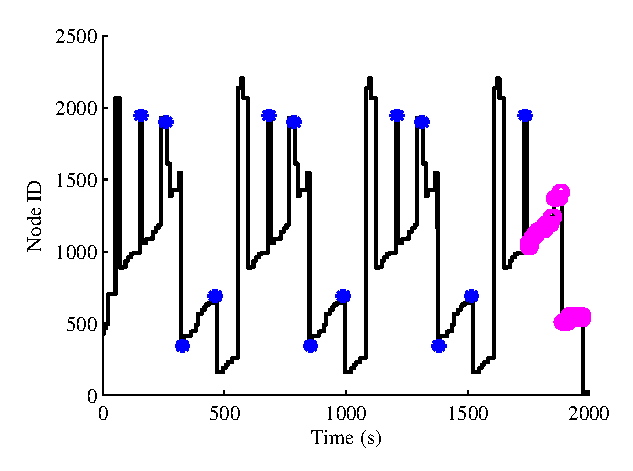
\includegraphics[width=3in]{graphics/AutRnd5_Sim8_nodes.eps}

    \caption[`LAGR' timid night watch automaton node switching.]{As the system
      executes, the automaton changes nodes based on the discrete inputs and
      inclusion of the current pose in a given policy domain.  The graph shows three
      distinct phases.  The thirteen points marked with '*' indicated the check
      points passed.  The thickest portion, which is actually closely spaced
      `$\circ$' symbols, shows the portion where the intruder is detected.  Notice
      that the system makes multiple passes past each checkpoint before the intruder
      is detected.}
   \label{fig:lagr_Aautomaton_full_nodes}
\end{figure}


\refig{lagr_Aautomaton_full_nodes} shows the progression of the system through the
automaton nodes as the system moves through the environment.  Note the cyclic nature
as the system completes three patrols before the intruder is detected.  As the
automaton state transitions, so does the associated policy as shown in
\refig{lagr_Aautomaton_full_policies}.

\begin{figure}[bt]
  \centering 
  \psfrag{3500}{3500}
  \psfrag{3000}{3000}
  \psfrag{2500}{2500}
  \psfrag{2000}{2000}
  \psfrag{1500}{1500}
  \psfrag{1000}{1000}
  \psfrag{500}{500}
  \psfrag{Time (s)}{Time (s)}
  \psfrag{Policy ID}{Policy ID}
  \psfrag{Policy}{}
   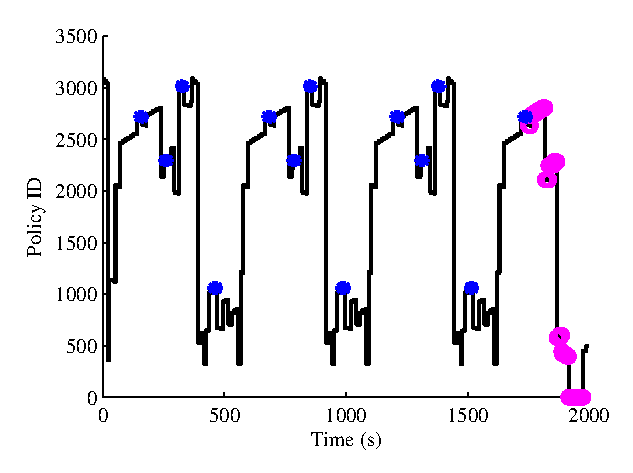
\includegraphics[width=3in]{graphics/AutRnd5_Sim8_policies.eps}

   \caption[`LAGR' timid night watch policy switching.]{Each node in
     the automaton is associated with a particular policy in the
     suite.  As the system executes, the local policies are activated
     by the automaton based on the local pose estimate.The graph shows
     the same three distinct phases as
     \refig{lagr_Aautomaton_full_nodes}.}
   \label{fig:lagr_Aautomaton_full_policies}
\end{figure}

In this execution strategy, the continuous evolution of the system governs the
discrete transitions in the automaton; therefore, the resultant transitions are
asynchronous, and not governed by a fixed time step.  In this current implementation,
the discrete inputs act as guards on the automaton transitions; the discrete input
must match the value associated with the child node to allow transition into the
child node, but does not force transition out of the current node.  Another approach
could check the discrete input at each update step and force transitions out of a
given automaton node if the inputs do not match the reference input.  This would
require that each node has a child with the same policy reference, but different
discrete inputs .

%\FloatBarrier

\begin{figure}[bt]
  \centering 
   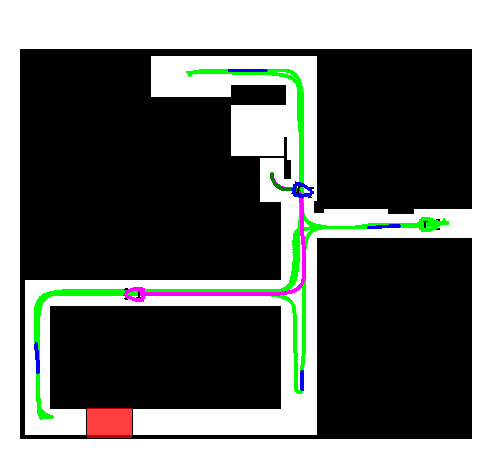
\includegraphics[width=3in]{graphics/AutRnd5_Sim7_path.eps}

   \caption[`LAGR' timid night watch re-planning.]{As new information
     becomes available, such the obstacle in the lower corridor, the
     automaton synthesis formulates a different automaton based on
     changes to the prepares graph.  The new automaton preserves the
     correct behavior.}
   \label{fig:lagr_Aautomaton_blocked}
\end{figure}


If the prepares graph changes, the automaton synthesis algorithm must be re-run.
\refig{lagr_Aautomaton_blocked} shows the simulated path taken when an automaton is
synthesized for the prepares graph with 24 policies associated with the lower
corridor invalidated.  The resultant automaton contains 2580 nodes; its execution
correctly satisfies the original specification by only invoking valid policies.

%\FloatBarrier

The automaton synthesis approach guarantees the correct behavior under very
reasonable assumptions.  First, the automata synthesis only returns an automaton if
the specification is realizable for the given policy suite and associated prepares
graph. Second, given a realizable specification, the algorithm is guaranteed to
produce an automaton such that all its executions satisfy the desired behavior {\bf
  if} the environment behaves as assumed.  The construction of the automaton is done
using LTL statements that encode admissible environment behaviors; if the environment
violates these assumptions, the automaton is no longer correct.  Since the
specifications encode the transitions allowed by the prepares relationship, the only
case in which the system pose is not in the domain of $\Phi_{k}$, or in any successor
$\Phi_{l}$, is if the environment behaved ``badly.''  That is, either some
disturbance caused the policies to violate the prepares relationship, or the
environment violated assumptions governing the allowable discrete inputs.  This later
case requires careful sensor design, with only those restrictions that are
necessary.  Either case invalidates the automaton.  In the event that a valid
transition does not exist, the automaton executive raises an error flag, and halts
the system.  A new plan must be requested.

Unfortunately, for real systems disturbances are a fact of life.  Policies may be
designed to be as robust as possible, but disturbances may still take the system out
of the domain of a currently executing policy.  Often these disturbances are simply
due to pose estimation updates as described above.  The hybrid control system should
have a method of recovery, which will likely require some knowledge of the hybrid
control system and task.  For the task described in this section, our approach is to
search the automaton as a list of nodes until a node whose associated policy contains
the current pose estimate and whose discrete input matches the current sensor value;
as is done for the initial condition. This works in this example because of the
cyclic nature of the task.  

A more fundamental problem is when the disturbance takes the system
outside the domain of all policies in the automaton.  Depending on the
initial specification, the automaton synthesis does not necessarily
use every available policy.  As with sequence-based approaches, this
has a negative impact on the overall robustness of the policy
composition technique relative to the collection of available
policies.  This thesis considers two approaches to addressing the
problem of unused policies.

The first approach explicitly allows the initial condition to be in any available
policy and have any allowable sensor value.  The assumption during synthesis that the
system is in one of two initial policy domains is made to limit the size of the
automaton.  No assumptions about the initial policies could be made such that
$\varphi_i^s=\NOT\STOP$; this would force the automaton to include all policies, but
would greatly increase the size of the synthesized automaton.  The particular
implementation of the synthesis algorithm used in this thesis precluded this
approach; this is not a theoretical issue, later work will build a more robust
synthesis tool to address this implementation issue~\cite{hadas_pc}.

The second approach, which is used in these experiments, is to augment the
synthesized automaton to add nodes for each unused policy/sensor combination.  If a
policy is unused by the original automaton, but prepares another policy that is used
for all input combinations, then a node is added to the automaton with the unused
policy as a reference.  This added node ignores the sensor inputs.  The children of
the added node are all nodes in the automaton whose associated policies are prepared
by the added node's policy or have the same policy reference.  Since all input
combinations are covered, a valid child transition will eventually exist.  This
process is repeated until all policies that prepare others are added to the
deployment.  This approach maximizes the overall hybrid control policy domain for the
given collection of domains, while adding the smallest number of nodes to the
automaton.  This gives the system a way to ``get back on track.''  If the disturbance
causes the system pose to exit the domains of every policy in the suite, then the
hybrid control policy will stop the robot and cease execution.  Only by adding
additional policies, and regenerating the automaton can the system recover.


\begin{figure}[bt]
  \centering 
   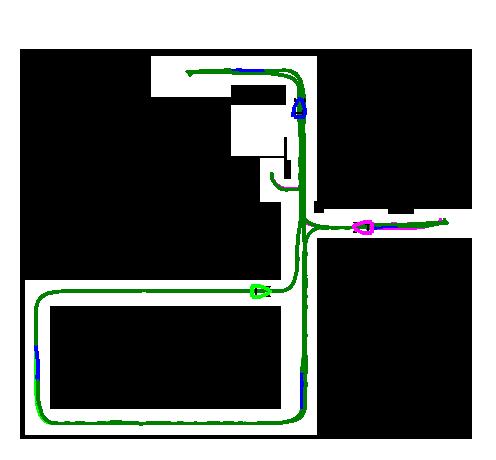
\includegraphics[width=3in]{graphics/AutRnd5_Run4_path.eps}

   \caption[`LAGR' timid night watch experiments.]{Actual run on
     LAGR robot.  Here, the robot resumes patrolling after hiding
     early in the experiment.}
   \label{fig:lagr_Aautomaton_experiments}
\end{figure}

\refig{lagr_Aautomaton_experiments} shows an example run using the augmented
automaton.  During the experimental runs, the intruder is signaled at will via a
switch on the remote control used an emergency stop.  The experiment successfully
satisfies the specification.  \refig{lagr_Aautomaton_experiments_nodes} shows the
progression of nodes during execution.  Note that the nodes above 2400 are augmented
nodes; without these, the execution would have ceased earlier due to disturbances.
Given the augmented automaton, the system is able to search for a node whose policy
contains the current pose.  Eventually, the execution did quit when a disturbance
finally took the system out of the domain of all the policies.
\refig{lagr_Aautomaton_experiments_policies} shows the policy switching induced by the
augmented automaton.  The experiment was repeated several times; the automaton
successfully induced the correct behavior each time until disturbances caused the
system to terminate; this points to the need for more policies to be added to the
policy suite.

\begin{figure}[bt]
  \centering 
  \psfrag{3500}{3500}
  \psfrag{3000}{3000}
  \psfrag{2500}{2500}
  \psfrag{2000}{2000}
  \psfrag{1500}{1500}
  \psfrag{1000}{1000}
  \psfrag{500}{500}
  \psfrag{Time (s)}{Time (s)}
  \psfrag{Node ID}{Node ID}
  \psfrag{Automaton Nodes}{}
   \includegraphics[width=3in]{graphics/AutRnd5_Run4_nodes.eps}

   \caption[`LAGR' node switching during experiment]{Node switching with
     invocations of augmented nodes shown by 'x'; the controller would have ceased
     execution were it not for these added nodes.}
   \label{fig:lagr_Aautomaton_experiments_nodes}
\end{figure}



\begin{figure}[bt]
  \centering 
  \psfrag{3500}{3500}
  \psfrag{3000}{3000}
  \psfrag{2500}{2500}
  \psfrag{2000}{2000}
  \psfrag{1500}{1500}
  \psfrag{1000}{1000}
  \psfrag{500}{500}
  \psfrag{Time (s)}{Time (s)}
  \psfrag{Policy ID}{Policy ID}
   \psfrag{Policy}{}
  \includegraphics[width=3in]{graphics/AutRnd5_Run4_policies.eps}

   \caption[`LAGR' policy switching during experiment]{Policy switching during an experiment.}
   \label{fig:lagr_Aautomaton_experiments_policies}
\end{figure}

The drawback to the augment and search approach is that there is no history;
therefore, the system will sometimes repeat an earlier portion of the patrol loop,
prior to visiting the other nodes.  This problem could be addressed by adding an
output that encodes which ``downstream'' check point will be encountered next, and
using this information to guide the search for a valid node.  This requires
associating each policy with the closest checkpoint before the synthesis.  One
possible approach is to choose the checkpoint that generates the least cumulative
cost for a given policy from a set of costs generated by considering each checkpoint
as the goal of a total ordering.  During disturbance recovery, the system searches
for a node whose associated policy domain contains the current pose and whose
``ClosestCheckpoint'' output matches the assigned checkpoint for that policy.

%\FloatBarrier%afterpage{\clearpage}

The automata-base approach is capable of producing complex behaviors, which allow the
system to react to changes in the environment via the binary environmental inputs.
Additionally, the automata-based approach allows the system to exhibit desirable
limit cycles; in this example, repeatedly patrolling a hallway.  Thus automata-based
approaches are more suitable for repetitive tasks than order-based approaches.  That
said, the automata should make use of all available policies, and provide a method of
recovery, in order to maintain robustness to disturbance that is the hallmark of
order-based approaches.

% \subsection{Ackermann Steered Car-like Parking Simulations}
% \label{sec:automaton_ackermann_automaton}

% \begin{figure}[bt]%[ht]
% \begin{center}

%  \vspace{0.2in}

%  \includegraphics[width=4in]{graphics/sim_parking_demo.eps} 

%   \caption[Local parking behavior induced by meta-policy]{Parking behavior induced by
%     the composition of local policies.  The feedback control policies guarantee the
%     safety of the maneuver.}
% \label{fig:automata_parking}
% \end{center}
% \end{figure}

% This section provides an example of policy-based planning with the more complex
% system model of an Ackermann steered car.  Here, the scenario is one of searching for
% an available parking space, and then parking.  The environment is known; what is
% unknown is whether a given parking space is available or occupied.  The system has a
% local sensor for detecting open parking spaces; thus, the system must search for an
% available parking space by systematically driving past all the parking spaces.  If an
% open parking space is found, the system changes behavior from searching to parking,
% and executes the parking maneuver as illustrated in \refig{parking}.  The results
% demonstrate coupled planning and control for a complex system that exhibits complex
% behaviors that change based on reactions to the changing environment.

% \begin{figure}[bt]
%   \centering
%   \includegraphics[width=0.75\linewidth]{graphics/sim_parking_run_0_world.eps}
%   \caption[Environment for parking simulations]{The environment has 40 parking spaces
%     arranged around the middle city block.  Initially, there are five empty parking
%     spaces randomly chosen in the environment.}
%   \label{fig:automaton_acker_parking_world}
% \end{figure}

% The environment, shown in \refig{automaton_acker_parking_world}, consists of two city blocks
% accessible from ten entering roads.  Each road consists of two lanes that follow the
% American standard of driving on the right side.  One block is surrounded by 40
% parking spaces; 20 for the clockwise direction and 20 for the counterclockwise
% direction. The entry/exit points are labeled 1-10 clockwise starting from the
% north/south lanes at the top left of the environment.  The parking spaces are
% identified with a numeric identifier adjacent to each space.  The roadway lanes and
% parking spaces are sized for an urban environment.  The robot system uses an
% Ackermann steered kinematic model that controls the forward velocity and the rate of
% steering angle change; see \reapp{robots} for details.

% \begin{figure}[bt]
%  \begin{center}
%  \begin{minipage}[b]{\linewidth}
%  \begin{minipage}[b]{0.48\linewidth}
%   \centering 
%   \includegraphics[width=\linewidth]{graphics/parkway_details_parking.eps}

%  {\scriptsize a) Policies for parking.}
%    \end{minipage}
%  \hspace{0.03\linewidth} % To get a little bit of space between the figures
%  \begin{minipage}[b]{0.48\linewidth}
%    \centering 
%    \includegraphics[width=\linewidth]{graphics/parkway_details_leaving.eps}

%   {\scriptsize b) Policies for leaving}
%  \end{minipage}

%  \end{minipage}
 
%  \caption[Parking policy details]{Details of policies used for parking
%    and leaving.  The policies, which are shown relative to the cache
%    reference point, are shown wider than normal to show details.  Six
%    policies are associated with parking.  Five policies are used to
%    exit a parking space and prepare policy in the traffic lane.}
%   \label{fig:automata_parkway_details}
% \end{center}
% \end{figure}

% The parking demonstrations use a collection of 16 \PF style policies, which are
% instantiated in the policy cache relative to the origin.  The cache includes policies
% for traveling straight down a roadway lane, for parking and leaving a given space,
% and for turning at intersections.  \refig{parkway_details} shows examples of the
% policies for parking and leaving, which treated as meta-policies for planning
% purposes.  Associated with the inlet policy of the parking policy is a sensor that
% determines whether the parking space is available.  If the parking space is
% unavailable, then the parking meta-policy prepares some other policy further down the
% roadway lane.  \refig{parkway_intersection} shows an example intersection, the
% deployed policies, and the extent of the robot body into the workspace.  Since this
% is a simulation, only those policies needed for basic traffic are deployed.  No
% attempt is made to fill the free pose space in order to provide robustness.


% \begin{figure}[bt]
%  \begin{center}
%  \begin{minipage}[b]{\linewidth}
%  \begin{minipage}[b]{0.48\linewidth}
%   \centering 
%   \includegraphics[width=\linewidth]{graphics/parkway_intersection_lanes.eps}

%   \end{minipage}
%  \hspace{0.03\linewidth} % To get a little bit of space between the figures
%  \begin{minipage}[b]{0.48\linewidth}
%    \centering 
%    \includegraphics[width=\linewidth]{graphics/parkway_intersection_padded.eps}

%  \end{minipage}

%  \begin{minipage}[b]{0.48\linewidth}
%   \centering 

%   {\scriptsize a) Connected policy domains projected into workspace}

%  \end{minipage}
%  \hspace{0.03\linewidth} % To get a little bit of space between the figures
%  \begin{minipage}[b]{0.48\linewidth}
%    \centering 

%    {\scriptsize b) Body extent over the policy domains}

%  \end{minipage}
%  \end{minipage}
 
%  \caption[Policies deployed at intersection]{Deployment of policies at an
%    intersection.  The polices include those that pass straight through the
%    intersection, as well as left and right turns.  Other policies are used to tie the
%    straight sections to the turns.  The policy domains, which are widened to increase
%    visibility, appear as thick lines in (a).  }
%   \label{fig:automata_parkway_intersection}
% \end{center}
% \end{figure}

% For the simulations in this section, a total of 306 policies are deployed in the
% environment.  The regularity of the environment allows an automated approach to
% policy instantiation based on a collection of reference points defined relative to
% the intersections and parking spaces.  The policy total includes 40 parking
% meta-policies and 40 leaving meta-policies, as well as 24 each left, right and
% straight maneuvers at the six intersections.  Policies to enter and leave the
% environment are added at the 10 roadways connecting the environment to the outside
% world.  Given the suite of 306 policies, the prepares graph is automatically defined
% as described in \resec{nonholo}.

% In many ways, the policy suite and prepares graph can be viewed as information that
% the environment communicates to the vehicle.  One can envision a scenario where this
% information is passed to a vehicle as the system enters a new neighborhood.  The
% vehicle could quickly verify that its system model and input constraints are valid
% for the policies defined in the cache; multiple suites and caches could be defined
% for a range of vehicle sizes.  Given a valid suite of policies, the vehicle is then
% free to plan its local behavior over this environment.

% %\FloatBarrier%afterpage{\clearpage}

% \subsubsection{Basic Parking Scenarios}
% \label{sec:automaton_acker_parking}

% The basic scenario considers a single car that must park in the
% environment.  The environmental input is a sensor called `\PARK' that
% tells the car if a parking space is available; the system output
% identifies which policy to activate.  The car may enter from any of
% the ten roadways connecting to the two blocks; that is
% $\varphi_i^s=\OR_{i\in\mrm{InitialPolicies}} \CP_i$.  Since these are
% not adjacent to a parking space, $\varphi_i^e = \NOT\PARK$.  The car
% can only determine whether there is a free parking space if we are in
% a policy next to it. This means that `Park' cannot become true if the
% vehicle is not next to a parking space or in one. Also, for
% implementation reasons, we assume that the input `Park' remains true
% after parking.
% $$\varphi_t^e = \left\{\begin{array}{c}
%     \ALWAYS\prl{\;\;\brl{\;\;\;\;\prl{\NOT \prl{\bigvee_{i\in \mrm{ParkPolicies}}\Phi_i}}\;\AND\; 
%         \prl{\NOT\prl{\bigvee_{j\in \mrm{PreparesParkPolicies}}\Phi_j}}}  
%       \Rightarrow\;\NOT\NEXT\PARK}\\
%     \AND\;\;\ALWAYS\prl{\;\prl{\PARK\,\AND\, \prl{\bigvee_{i\in \mrm{ParkPolicies}}\Phi_i}} \; 
%       \Rightarrow\;\NEXT\PARK\;} \end{array}\right.  $$ 
% We have no assumptions on the goals of the environment, and make no assumptions about
% the availability of an empty parking spot, therefore $\varphi_g^e = \Box \Diamond(TRUE)$. 

% The allowable system transitions are encoded as
% $$\varphi_t^s = \left\{\begin{array}{l}\bigwedge_i
%     \;\ALWAYS\prl{\Phi_i\;\Rightarrow\;\prl{\NEXT \Phi_i\bigvee_{j\in
%           \mrm{SuccessorsOfPolicy}_i}\NEXT \Phi_j}}\\ 
%     \bigwedge_{i\in \mrm{ParkPolicies}} \;\Box \prl{\NOT\NEXT\PARK\;\Rightarrow\;\NOT\NEXT \Phi_i}\\ 
%     \bigwedge \; \ALWAYS\prl{\NEXT\PARK\;\Rightarrow\;\prl{\bigvee_{i\in \mrm{ParkPolicies}}\NEXT \Phi_i}\;}    
% \end{array}\right.  $$
% %The vehicle can only transition from one policy to the next based on
% The first line encodes the transitions of the prepares graph.  The vehicle cannot
% park if there is no parking space available, as indicated by the `Park' input on the
% second line.  The third line states that if there is an empty parking space, the car
% must park; removing this line may allow the vehicle to pass an open spot before
% parking.

% The system goal encodes a list of policies the vehicle must visit
% infinitely often if it has not parked yet; thus,
% \[\varphi_g^s = \bigwedge_{i\in \mrm{VisitPolicies}}\ALWAYS
% \EVENTUALLY(\Phi_i\,\OR\,\PARK)\,.\] The list of `VisitPolicies'
% define the area in which the vehicle will look for an available
% parking space; in this case, the visit policies correspond to the
% eight lanes around the parking spaces (four going clockwise and four
% going counter clockwise).  Note, this goal condition is true if either
% the vehicle visits these policies infinitely often (when there is no
% parking space available) or it has parked.  Defining the
% `VisitPolicies' list in a different order would change the search
% strategy induced by the automaton.  Additional specifications could be
% written to tie the search strategy to the point of entry, but this
% would increase the size and complexity of the automaton.

% Defining proper specifications in LTL is something of an art.  Improper
% specifications may make the automaton unrealizable, which will require
% modifications to the specifications, or may lead to undesirable
% behaviors.  Ongoing research is attempting simplify the process by
% going from specifications written in structured English to the
% required LTL specification~\cite{hadas_iros_07}.  


%  \begin{figure}%[tb]
%    \begin{center}
%    \begin{minipage}[b]{\linewidth}
%    \begin{minipage}[b]{0.44\linewidth} 
%    \centering 
%    \includegraphics[width=\linewidth]{graphics/sim_parking_run_1_world.eps}   
  
%    \vspace{-1.6ex}
%    {\small Run \#1} 
%    \end{minipage}
%   \hspace{0.03\linewidth}
%   \begin{minipage}[b]{0.44\linewidth}
%    \centering  
%    \includegraphics[width=\linewidth]{graphics/sim_parking_run_2_world.eps} 
  
%    \vspace{-1.6ex}
%    {\small Run \#2}
%  \end{minipage} 
%  \end{minipage}  
%  \caption[Two executions of parking simulation]{Two executions of the basic parking
%    scenario.  The initial conditions for each run are circled. }
%     \label{fig:automaton_acker_parking_runs_12}

%  \end{center}
%  \end{figure}

%  \begin{figure}%[tb]
%    \begin{center}
%    \begin{minipage}[b]{0.44\linewidth} 
%    \centering 
%    \includegraphics[width=\linewidth]{graphics/sim_parking_run_3_world.eps}   
  
%    \vspace{-1.6ex}
%    {\small Run \#3} 
%    \end{minipage}
%   \hspace{0.03\linewidth}
%   \begin{minipage}[b]{0.445\linewidth}
%    \centering  
%    \includegraphics[width=\linewidth]{graphics/sim_parking_run_4_world.eps} 
  
%    \vspace{-1.6ex}
%    {\small Run \#4}
%  \end{minipage} 

%    \vspace{0.5ex}

%    \begin{minipage}[b]{0.44\linewidth} 
%    \centering 
%    \includegraphics[width=\linewidth]{graphics/sim_parking_run_5_world.eps}   
  
%    \vspace{-1.6ex}
%    {\small Run \#5} 

%    \end{minipage}
%   \hspace{0.03\linewidth}
%   \begin{minipage}[b]{0.44\linewidth}
%    \centering  
%    \includegraphics[width=\linewidth]{graphics/sim_looping_run_6_world.eps}
 
%    \vspace{-1.6ex}
%    {\small Run \#6}

%  \end{minipage} 

 
%  \caption[Four executions of parking simulation]{Four executions of the basic parking
%    scenario.  The initial conditions for each run are circled.  The last run
%    continues to loop as no parking spaces are available. }
%     \label{fig:automaton_acker_basicSim}

%  \end{center}
%  \end{figure}

% %\FloatBarrier

% For simulations shown in Figures~\ref{fig:automaton_acker_parking_runs_12}
% and~\ref{fig:automaton_acker_basicSim}, a new vehicle is introduced at a random entrance.  The
% parking spaces are filled according to the previous run.  As the automaton executes,
% if a parking policy is a successor to the current state, the empty/occupied status is
% checked via the local `Park' sensor. This work does not address the required sensor,
% but assumes a binary output.  Transition to the parking policy is enabled if the
% associated space is empty.  If the transition is enabled, `Park' remains true so that
% other transitions are disabled until the vehicle pose enters the domain of the
% parking meta-policy, and the system parks.  Six runs are simulated using the global
% parking automaton; The first five runs park.  In Run \#6, there are no parking spaces
% available; therefore, the vehicle continues to circle past every possible parking
% space, waiting on another vehicle to leave.

% \subsection{Multi-vehicle Scenarios}
% \label{sec:automaton_acker_multi_car}

% The automata-based approach to policy composition naturally extends to multi-agent
% systems~\cite{hadas_07}.  The local policies guarantee predictable local behavior of
% a single agent; the automata governs the switching between local policies to
% coordinate the high-level behavior of an agent.  Taking this approach further,
% Kress-Gazit \ea~\cite{hadas_07} use the environmental inputs to coordinate behavior
% between agents using automata.  Each agent runs its own automata-based hybrid
% controller, which responds to other agents via environmental inputs; that is, the
% outputs of one agent become inputs to another agent.  This section details a
% simulation using the policy composition approach advocated in this thesis with the
% automata-based multi-agent coordination scheme advocated in~\cite{hadas_07}.  The
% simulation results illustrate several issues that arise with this approach.

% In order to expand the basic parking approach to allow for multiple vehicle
% scenarios, the LTL formulas from above are modified.  The approach uses an additional
% input and several outputs.  The additional input is `Hazard', which causes the
% vehicle to stop in place.  The hazard can be triggered by proximity to another
% vehicle, or by an external device such as a stop-light.  When the hazard clears, the
% robot should resume motion as before.  In a real system, many hazards can be avoided
% by slowing down, and waiting for the other vehicle to clear.  For simplicity, these
% simulations require the system to stop.  When the vehicle stops in response to a
% `Hazard', the system outputs `\STOP'.  Additional outputs signal `\LEFT' and `\RIGHT'
% as appropriate.  There are also outputs that signal the vehicles intentions for
% `Parking' and `Leaving'.  The automaton outputs can be sensed by other vehicles in
% the environment.

% The LTL specifications from above are modified to take the new inputs
% and outputs into consideration, and allow a new ``leaving'' behavior.
% Each vehicle in the simulation runs a local copy of one of two
% automata.  The only coordination is via the individual `Hazard'
% sensor.  We now consider each automaton in turn.

% \paragraph{Parking Automaton}
% The parking automaton for the multi-vehicle scenario is similar to the
% individual case, but includes the stopping behavior and the additional
% outputs.  The initial environment inputs are given by $\varphi_i^e =
% \NOT\PARK\,\AND\,\NOT\HAZ$.  The initial system outputs are given by
% $\varphi_i^s=\bigvee_{i\in\mrm{InitialPolicies}} \CP_i\,\AND\,
% \NOT\LEFT\,\AND\, \NOT\RIGHT\,\AND\,\NOT\STOP\,\AND
% \,\NOT\PARKING\,\AND\,\NOT\LEAVING$.  The environmental transitions
% encoded by $\varphi_t^e$ are the same as for the individual case; that
% is, the `Park' input can only become true adjacent to a parking
% policy, and remains true after the input\footnote{This could cause
%   problems if another car prevents the car from parking by approaching
%   too close; this simulation assumes the `Hazard' input enforces a
%   ``courteous behavior.''}.  The system transitions include all the
% conditions of the individual parking case, plus the conditions that
% activate the outputs for turning, stopping, or parking as needed;
% thus,
% $$\varphi_t^s = \left\{\begin{array}{l}
% \bigwedge_i\;\ALWAYS\prl{\Phi_i\;\Rightarrow\;\prl{\NEXT \Phi_i\bigvee_{j\in\mrm{SuccessorsOfPolicy}_i}\NEXT \Phi_j}}\\ 
% \bigwedge_{i\in \mrm{ParkPolicies}} \;\Box \prl{\NOT\NEXT\PARK\;\Rightarrow\;\NOT\NEXT \Phi_i}\\ 
% \bigwedge \; \ALWAYS\prl{\NEXT\PARK\;\Rightarrow\;\prl{\bigvee_{i\in \mrm{ParkPolicies}}\NEXT \Phi_i}\;}\\
% \bigwedge \; \ALWAYS\prl{\prl{\bigvee_{j\in\mrm{LeftTurnPolicies}}\NEXT\CP_j}\,\IFF\,\NEXT\LEFT}\\
% \bigwedge \; \ALWAYS\prl{\prl{\bigvee_{j\in\mrm{RightTurnPolicies}}\NEXT\CP_j}\,\IFF\,\NEXT\RIGHT}\\
% \bigwedge \; \ALWAYS\prl{\NEXT\HAZ\,\IFF\,\NEXT\STOP}\\
% \bigwedge \; \ALWAYS\prl{\prl{\NEXT\PARK\,\AND\,}\,\IFF\,\NEXT\PARKING}\\
% \end{array}\right.\,\,.  $$
% The system goal is given by
% \[\varphi_g^s = \bigwedge_{i\in \mrm{VisitPolicies}}\ALWAYS
% \EVENTUALLY\prl{\Phi_i\,\OR\,\PARK\,\OR\,\STOP}\,.\] The goal
% condition allows for a vehicle to remain stopped if a broken stop-light
% or accident ahead blocks the roadway.  With these specifications, the
% parking automaton has 2142 nodes.


% \paragraph{Leaving Automaton}
% In this scenario, a vehicle is leaving its parking space and exiting the block via
% some specified exit. The leaving automaton for the multi-vehicle scenario has an
% extra input that specifies which of the ten possible exits the vehicle will exit; let
% $\crl{\mrm{Exit}\CP_i}$ denote a set of binary propositions that are true if the
% associated exit is selected, and false otherwise.  The initial environment
% specification is
% \[\varphi_i^e = \NOT\HAZ\,\AND\,\prl{\bigvee_{i\in\mrm{ExitPolicies}}\;
%   \left(\mrm{Exit}\Phi_i \bigwedge_{j\in \mrm{ExitPolicies}, j\neq
%       i}\NOT\mrm{Exit}\CP_j\right)}\,,\] that is, only one exit is specified.  Two
% different vehicles leaving two different parking spots may use the same synthesized
% automaton with different inputs that designate the desired exit.  We require the exit
% specification to be constant, meaning it cannot change once it is given; therefore,
% the system transition is specified as $\varphi_t^e = \bigvee_{i\in
%   \mrm{ExitPolicies}}\;\left(\mrm{Exit}\CP_i \;\IFF\; \NEXT\mrm{Exit}\CP_i
% \right)\,.$ We make no assumptions on the infinite behavior of the environment,
% therefore the goal component remains set to true; that is $\varphi_g^e =
% \ALWAYS\EVENTUALLY\TRUE$.  Initially, the car is leaving a parking space, hence it
% must turn on the left turn signal; thus,
% \[\varphi_i^s = \left\{\bba{l}
% \bigvee_{i\in \mrm{LeavingPolicies}} \CP_i \\
% \AND\,\LEFT\,\AND\, \NOT\RIGHT \,\AND\, \LEAVING 
%   \,\AND\,\NOT\PARKING \,\AND\, \NOT\STOP
% \eba\right.\,.\]  
% The system transitions are given by
% \[\varphi_t^s = \left\{\begin{array}{l}
% \bigwedge_i\;\ALWAYS\prl{\Phi_i\;\Rightarrow\;\prl{\NEXT \Phi_i\bigvee_{j\in\mrm{SuccessorsOfPolicy}_i}\NEXT \Phi_j}}\\ 
% \bigwedge \; \ALWAYS\prl{\prl{\bigvee_{j\in\mrm{LeftTurnPolicies}}\NEXT\CP_j}\,\IFF\,\NEXT\LEFT}\\
% \bigwedge \; \ALWAYS\prl{\prl{\bigvee_{j\in\mrm{RightTurnPolicies}}\NEXT\CP_j}\,\IFF\,\NEXT\RIGHT}\\
% \bigwedge \; \ALWAYS\prl{\NEXT\HAZ\,\IFF\,\NEXT\STOP}\\
% \bigwedge \; \ALWAYS\prl{\prl{\NEXT\prl{\bigvee_{i\in\mrm{LeavingPolicies}}\CP_i}}\,\IFF\,\NEXT\LEAVING}\\
% \end{array}\right.\,\,.\]
% The system goal is specifies that the vehicle must go to the designated exit policy
% unless it stops; that is
% $$\varphi_g^s = \bigwedge_{i\in ExitPolicies}\ALWAYS\EVENTUALLY\prl{\; 
%   \prl{\Phi_i\Leftrightarrow Exit\Phi_i}\;\OR\,\STOP}$$ 
% With these specifications the leaving automaton has 1908 nodes.

% The key to using these automata in a decentralized multi-agent scenario is the
% coordination provided by the `Hazard' sensor.  Each vehicle executes its own hazard
% sensor with a single binary value `Hazard.'  The `Hazard' input is based on either a
% timed stop-light or a proximity/precedence sensor.  The stop-light alternates between
% north/south and east/west travel along the roadways.  Each intersection transitions
% at the same time; there is a slight overlap where all directions are stopped.  Any
% vehicle entering the policies just before the left/right/straight policies at each
% intersection checks the current value of the stop-light.  If the ``red light'' is
% visible, the `Hazard' flag is set to TRUE.

% The `Hazard' sensor is a discrete hybrid automaton in its own right, that attempts to
% determine precedence based on the robot's internal state and binary outputs, and the
% other robots relative pose, velocity, and binary outputs.  Thus the ``sensor'' is a
% mixture of continuous measurements and discrete logic.  The `Hazard' checks proximity
% of other vehicles, and determines the precedence relationships between vehicles; that
% is, which vehicle must yield to the other.  For this simulation, the `Hazard' sensor
% is hand-coded and tuned to given the proper performance.  The sensor automaton sets
% `Hazard' to true whenever the car is too close to a car ahead of it (keeping safe
% distance), whenever a car ahead is backing up to park (being polite), whenever the
% car is leaving a parking space and another car passes by and whenever another car is
% leaving a parking space which the car will park in next.  In this decentralized
% coordination scheme, each vehicle's `Hazard' sensor must infer the intentions of the
% others based their outputs.  There is no centralized communication of intentions.

% \begin{figure}[bt]%[tb]
%   \begin{center}
%   \begin{minipage}[b]{0.45\linewidth} 
%   \centering 
%   \includegraphics[width=0.9\linewidth]{graphics/sim_hazard_run_7a.eps} 
  
%   {\small Run \#7 - a} 

%   \end{minipage}
%  \hspace{0.03\linewidth}
%  \begin{minipage}[b]{0.45\linewidth}
%   \centering  
%   \includegraphics[width=0.9\linewidth]{graphics/sim_hazard_run_7b.eps} 

%   {\small Run \#7 - b}
% \end{minipage} 

% \caption[Simple multi-vehicle traffic simulation]{In this continuation of Run \#6,
%   the two snap shots show a simple multiple vehicle scenario.  A timed stop-light
%   triggers a `hazard' input that causes the vehicle heading east to stop.  This
%   allows the vehicle from Run\#6 to travel through the intersection, and eventually
%   park in the newly available parking spot.}
%    \label{fig:automaton_acker_multipleSim}

% \end{center}
% \end{figure}

% \refig{automaton_acker_multipleSim} shows the continuation of Run \#6 with the
% hazard inputs added to the parking automaton, and the new leaving
% automaton controlling the second vehicle.  In the first snapshot,
% vehicle \#6 is just beginning to approach the intersection, while
% vehicle \#7 stops for the light.  The second snapshot shows vehicle
% \#7 dutifully waiting for the signal, while vehicle \#6 has passed
% through the intersection.  Although not shown, after the stop-light
% changes, vehicle \#7 exits the area and vehicle \#6 continues around
% under the control of the global parking automaton and parks in the
% newly open spot.

% %\FloatBarrier

% \begin{figure}[bt]
%   \centering
%   \includegraphics[width=0.60\linewidth]{graphics/sim_parking_run_5_t1591.eps}
%   \caption[Snapshot of complex multi-vehicle traffic simulation]{A snapshot of a more
%     complex multi-vehicle simulation.  Each vehicle executes an
%     automaton that encodes the high-level specification ``stop on
%     hazard'' and either ``drive around until you find a free parking
%     space and then park'' or ``leave your parking space and exit the
%     block''.  Coordination between robots is done via an individual
%     `Hazard' sensor in a decentralized approach.  This snapshot is
%     taken at 15.91 seconds.}
%   \label{fig:automaton_acker_multi_run1}
% \end{figure}

% \refig{automaton_acker_multi_run1} shows an example of a more complex multi-vehicle simulation.
% At this point in time, seven cars are moving in the workspace.  Initially, 35 of the
% 40 parking spaces were randomly specified as occupied.  In this simulation, eight
% cars enter the block at different times and from different entry points, looking for
% a parking space. The times and entry points are (t=0.06 seconds, Entry = 10),
% (1.0,2), (2.0,7), (5.0,8), (7.0, 5), (10.0,6), (15.0, 8), (22.0,5).  During the
% execution, three cars leave their parking spaces and exit the workspace.  The times,
% parking spaces, and exit point are (t=13.0, Parking=23,exit=1), (15.0, 6, 7), and
% (30.0, 32, 5).  The simulation runs until 76.33 seconds of elapsed time when the last
% car exits or is parked.  \refig{simGeneral} shows a general snapshot of the
% simulation at a later time.  Cars whose `Stop' output is true are marked with red
% ellipses; that is, those cars who stop because the `Hazard' input is true.  The three
% stopped cars in \refig{simGeneral} are obeying stop-lights.

% \begin{figure}[bt]
%   \centering
%   \includegraphics[width=0.6\linewidth]{graphics/sim_parking_run_5_t3133_Haz.eps}
%   \caption[Later snapshot of multi-vehicle simulation]{A later
%     snapshot taken at 31.33 seconds during the simulation. In this
%     figure, cars surrounded by red ellipses are cars that are stopping
%     due to the `Hazard' input signaled by the timed stop-light.}
%   \label{fig:simGeneral}
% \end{figure}

% %\FloatBarrier

%  \begin{figure}[bt]
%    \begin{center}
%    \begin{minipage}[b]{\linewidth} 
%    \begin{minipage}[b]{0.45\linewidth} 
%    \centering 
%    \includegraphics[width=\linewidth]{graphics/sim_parking_run_5_t1591_Haz_close.eps}   
% %  
%    \vspace{0.4ex}
%    {\small (a) Blue car leaving (t=15.91 s)} 
%    \end{minipage}
%   \hspace{0.03\linewidth}
%    \begin{minipage}[b]{0.431\linewidth} 
%    \centering 
%    \includegraphics[width=\linewidth]{graphics/sim_parking_run_5_t3469_Haz_close.eps}   
% %  
%    \vspace{0.4ex}
%    {\small (b) Red car parking (t=34.69 s)} 
% %
%    \end{minipage}
%    \end{minipage}
%  %

%    \vspace{0.8ex}

%    \begin{minipage}[b]{\linewidth} 
%    \begin{minipage}[b]{0.46\linewidth}
%    \centering  
%    \includegraphics[width=\linewidth]{graphics/sim_parking_run_5_t1629_Haz_close.eps} 
% %
%    \vspace{0.4ex}
%    {\small (c) Yielding to turn in progress (t=16.29s)}
%  \end{minipage} 
%   \hspace{0.03\linewidth}
%    \begin{minipage}[b]{0.45\linewidth} 
%    \centering 
%    \includegraphics[width=\linewidth]{graphics/sim_parking_run_5_t2641_Haz_close.eps}   
% %  
%    \vspace{0.4ex}
%    {\small (d) Two cars parking (t=26.41s)} 
% %
%    \end{minipage}
%    \end{minipage}
% %
%   \vspace{0.8ex}
% %
% %  
%     \begin{minipage}[b]{\linewidth} 
%  \begin{minipage}[b]{0.45\linewidth}
%    \centering  
%    \includegraphics[width=\linewidth]{graphics/sim_parking_run_5_t2718_Haz_close.eps}
% % 
%    \vspace{0.4ex}
%    {\small (e) Two cars parking (t=27.18)}
% %

%  \end{minipage} 
%   \hspace{0.03\linewidth}
%   \begin{minipage}[b]{0.45\linewidth}
%    \centering  
%    \includegraphics[width=\linewidth]{graphics/sim_parking_run_5_t4639_Haz_close.eps}
% % 
%    \vspace{0.4ex}
%    {\small (f) Two cars at stop-light (t=46.39s)}
% %
%  \end{minipage} 
%  \end{minipage} 
% %
 
%  \caption[Close up of multi-vehicle behaviors]{Close up looks at different behaviors
%    seen throughout the simulation.  }
%     \label{fig:aker_multi_SimClose}
% %
%  \end{center}
%  \end{figure}

%  \refig{aker_multi_SimClose} shows several close up looks at different traffic
%  behaviors encountered during the simulation. In (a), the blue car which is leaving
%  the parking space has stopped, indicated by a red ellipse, to let the brown car
%  drive by. This `Hazard' was invoked based on a ``proximity sensor.'' In (b), red car
%  is parking while the blue car waits for it to finish before passing.  In (c), the
%  orange car is stopping to allow the gray car to complete a left turn, according to
%  the precedence established by the individual car's `Hazard' sensors.  The white car
%  on the left is leaving the parking space that later will be occupied by the brown
%  car. Figures~\ref{fig:aker_multi_SimClose}-d and (e) are two snapshots of two cars
%  parking simultaneously in opposite lanes. The car that started the parking maneuver
%  later (bottom lane) pauses to allow the other car to park safely.
%  \refig{aker_multi_SimClose}-f shows two cars stopping before a stop-light. While the
%  white car stopped based on the stop-light, the black car behind stopped based on the
%  proximity to the car ahead of it.

%  Sensors, or more specifically the binary inputs used by the automaton, are
%  fundamental to the success of this decentralized approach.  First, as mentioned
%  above, the sensors must satisfy the assumptions made about them in the LTL formulas
%  for the environment; otherwise the automaton will not be correct. Failing to trigger
%  `Hazard' may allow collision as the local policies do not consider obstacle
%  avoidance.  Second, even if the sensors do satisfy these assumptions, they may still
%  cause correct, yet unintended behavior. For example, if the proximity sensor set the
%  `Hazard' input to true whenever another vehicle was in a certain radius, even if the
%  other vehicle was behind in a forward driving lane, both vehicles may get
%  deadlocked; that is, both would stop forever.  While this behavior satisfies the
%  original specification, it does not follow the spirit of finding a parking space.
%  On the other hand, both cars stopping might be a desired behavior when an accident
%  occurred, therefore we would not want to forbid it in the specifications.
 
%  Currently, there are no guarantees that the implemented `Hazard' sensor automaton is
%  correct in all cases, and will not introduce deadlock.  Such unintended behavior
%  would not be present in a centralized approach where the controller has full
%  knowledge and not just local information as is the case here; however, the
%  centralized approach does not scale well.  The decentralized approach, which does
%  scale well for additional robots, may deadlock for a poorly designed hazard sensor;
%  thus, much work remains to develop automatic ways of specifying the `Hazard' sensor
%  automaton and prove that the composition of these multiple automata is free of
%  deadlock.
%  %This is a classical problem in concurrent systems; fairness
%  %assumptions must be imposed on the inputs to ensure that the system
%  %will not deadlock.



\section{Conclusion}
\label{sec:concl}
 
\paragraph{Benefits of Policy Composition}
Since the hybrid control policy is based on local feedback control policies, the
overall controller inherits the properties of the individual policies.  This allows
the individual policies to be tuned to local conditions, whether to provide safety or
enhanced performance.  The local policies, in order to be composable, have provable
convergence guarantees, and retain the robustness to disturbances that is the
hallmark of feedback control.  The local feedback control policies are designed to be
memoryless, and allow for real time control.  Because each local policy has an
explicit domain, the hybrid control approach is inherently safe.  If a disturbance
takes the system outside the domains of all policies, the robot is halted and
execution of the hybrid control policy terminates.

By planning in the space of control policies using the prepares graph, the planning
becomes very flexible with regard to task.  This approach opens the door to formal
synthesis of hybrid feedback controllers for complex systems; for example the parking
controller demonstrated in \rechap{planning}.
%The size of the prepares graph is typically smaller than that required by a
%conventional grid-based planner for the same navigation problem; thus, the speed of
%planning and re-planning will be faster.  
The approach allows analysis of the reachability of a goal, or realizability of a
specification, with a given policy suite during the discrete planning phase, prior to
execution.

Using automata to execute the local feedback policies allow the
systems to exhibit complex, multi-task behaviors.  The approach
enables tasks to be specified at a high-level, and then executed in a
continuous manner, using a hybrid control policy synthesized from the
suite of local control policies and associated prepares graph.
Repetitive tasks are naturally encoded in the framework, which allows
the approach to induce limit cycle type behaviors.


\subsection{Extension of Planning Tools}
\label{sec:extend_planning}

The demonstrations provided in this thesis highlight the power and flexibility of the
policy composition approach.  They also point to several shortcomings that should be
addressed in the discrete planning domain.  Addressing these issues will increase the
power of the policy composition approach for the policies and systems described
above.  
%In some cases, there may be existing techniques that may be brought to bear
%on synthesis of hybrid control policies for robotics.

\paragraph{Sensor Automata and Composition}
The automata synthesis approach described in \rechap{planning} depends on sensors
that provide binary signals to the automata during run time.  As with the `Hazard'
sensor, these ``sensors'' are often hybrid automata in their own right.  That is, the
binary sensor values depend on a mixture of continuous variables and discrete logic.
Defining these sensors is currently done on an \emph{ad hoc} basis.  Techniques are
needed to synthesize these sensor automata, and prove that the composition of
multiple sensor and control automata are valid, and preserve the desired
specifications and liveness conditions.  An example, taken from the simulations in
this thesis and the DARPA Urban Grand Challenge (UGC), is the need to resolve
precedence at intersections and four-way stops.  Formal synthesis methods coupled
with local policy composition offers a way to automate what is currently a labor
intensive, error prone process; as evidenced by the failures of most of the teams
that entered the DARPA UGC.

\paragraph{Formal Recovery Methods and Global Synthesis}
Disturbances are a fact of life.  Thus, the automata synthesis should include all
available policies to maximize the domain over which the automata is valid, and have
a formal method of recovery.  For the repetitive behaviors, such as patrolling,
demonstrated in this thesis, it is sufficient to augment the automata with unused
policies, and then search for a node that had the correct discrete sensor values and
whose associated policy contained the current pose.  A more complex scenario, such as
the mail delivery robot, will require a more formal recovery approach to allow the
system to recover gracefully.  Instead of an \emph{ad hoc} approach, a formal and
automated approach to defining a recovery strategy is desired.  The recovery approach
should also include all policies to maximize the domain.

\paragraph{Automata Synthesis with Heuristic Costs}
A major shortcoming of the automata synthesis approaches demonstrated in this thesis
is that they do not consider heuristic costs.  Within a given policy suite, there may
be many policy combinations that will address a given scenario.  In fact, this is
desirable for maximum planning flexibility.  The synthesis approach needs to be able
rank different policy choices based on their relative cost.  Current techniques only
consider the number of transitions made, that is the number of edges traversed in the
graph walk, when choosing policies.  The focus of current techniques is on dealing
with the state explosion problem using efficient data structures such as Binary
Decision Diagrams (BDD)~\cite{Bryant_86,clarke_99}.  There has been some work in
combining BDDs with heuristic search; for example, consider the Set\{A*\}
approach~\cite{jensen_02}.  That work may prove fruitful for automata synthesis
research.

\paragraph{Automata Synthesis with Non-deterministic Outcomes}
The automata synthesis used in this thesis only considered deterministic prepares
graphs.  This eliminated the use of the extended prepares relationship.  There has
been some work on defining sequence based approaches which allow non-deterministic
prepares graphs~\cite{kloetzer_07}; however, the synthesis techniques for reactive
automata do not allow non-deterministic transitions at this time.

\paragraph{Automata Synthesis with Hybrid Stability Analysis}
The stability of the order-based hybrid policies is based on the assumption of
monotonic policy switching.  With automata, limit cycles are allowed.  In the hybrid
systems community, it is well known that switching between stable vector fields can
induce instability~\cite{Branicky:98b,decarlo_00,liberzon_99}.  While this is not an
issue for the kinematic systems addressed in this thesis, stability analysis will be
fundamental to more complex systems.  There are several approaches to analyzing the
stability of existing hybrid systems~\cite{Branicky:98b,decarlo_00,liberzon_99};
however, going in reverse, the synthesis problem must address this issue during
construction.

\vspace{0.5in}

To conclude, this thesis advocates an approach to specifying robot controllers that
respects low-level constraints by design, and provides a natural interface for
specifying user intentions.  Low-level feedback control policies induce local
behaviors in a guaranteed manner.  The user interacts at a high-level to specify
intended behaviors.  The robot then automatically synthesizes a hybrid control policy
that can realize the intention, or reports that the goal is not realizable for the
current collection of policies and initial condition.  The hybrid control policy
inherits the desirable properties of the local feedback policies, while guaranteeing
the high-level behaviors.  This approach, which is demonstrated on a class of
nonholonomically constrained systems in this thesis, is widely applicable, and
likely necessary for the dynamically capable robots of the future.






\appendices
%\section*{Appendix: Policy Design Details}
%Appendix one text goes here.

% % use section* for acknowledgement
% \section*{Acknowledgment}


% The authors would like to thank...


% Can use something like this to put references on a page
% by themselves when using endfloat and the captionsoff option.
\ifCLASSOPTIONcaptionsoff
  \newpage
\fi



% trigger a \newpage just before the given reference
% number - used to balance the columns on the last page
% adjust value as needed - may need to be readjusted if
% the document is modified later
%\IEEEtriggeratref{8}
% The "triggered" command can be changed if desired:
%\IEEEtriggercmd{\enlargethispage{-5in}}

% references section

% can use a bibliography generated by BibTeX as a .bbl file
% BibTeX documentation can be easily obtained at:
% http://www.ctan.org/tex-archive/biblio/bibtex/contrib/doc/
% The IEEEtran BibTeX style support page is at:
% http://www.michaelshell.org/tex/ieeetran/bibtex/
\bibliographystyle{IEEEtran}
% argument is your BibTeX string definitions and bibliography database(s)
\bibliography{IEEEabrv,dcc_hkg}
%
% <OR> manually copy in the resultant .bbl file
% set second argument of \begin to the number of references
% (used to reserve space for the reference number labels box)
% \begin{thebibliography}{1}

% \bibitem{IEEEhowto:kopka}
% H.~Kopka and P.~W. Daly, \emph{A Guide to \LaTeX}, 3rd~ed.\hskip 1em plus
%   0.5em minus 0.4em\relax Harlow, England: Addison-Wesley, 1999.

% \end{thebibliography}

% biography section
% 
% If you have an EPS/PDF photo (graphicx package needed) extra braces are
% needed around the contents of the optional argument to biography to prevent
% the LaTeX parser from getting confused when it sees the complicated
% \includegraphics command within an optional argument. (You could create
% your own custom macro containing the \includegraphics command to make things
% simpler here.)
%\begin{biography}[{\includegraphics[width=1in,height=1.25in,clip,keepaspectratio]{mshell}}]{Michael Shell}
% or if you just want to reserve a space for a photo:

\vspace{-0.5in}

\begin{IEEEbiography}[{\includegraphics[width=1in,height=1.25in,clip,
    keepaspectratio]{conne}}]{David~C.~Conner} (M '00) received the
  Ph.D. in Robotics from Carnegie Mellon University in 2007; he
  received the M.S. in Robotics in 2004.  His research interests
  include applications of differential geometry, hybrid systems, and
  control theory for mobile robot navigation and control.  He
  graduated with B.S.\ and M.S.\ degrees in Mechanical Engineering
  from Virginia Tech (VPI\&SU) in 1991 and 2000 respectively.  He is
  currently a research scientist with TORC Technologies in Blacksburg,
  Virginia.
\end{IEEEbiography}

\vspace{-0.2in}

\begin{IEEEbiography}[{\includegraphics[width=1in,height=1.25in,clip,
    keepaspectratio]{conne}}]{Hadas~Kress-Gazit} (M '??) received the
  Ph.D.\ in Mechanical Engineering from the University of Pennsylvania
  in 2008.

\end{IEEEbiography}

% You can push biographies down or up by placing
% a \vfill before or after them. The appropriate
% use of \vfill depends on what kind of text is
% on the last page and whether or not the columns
% are being equalized.

%\vfill

% Can be used to pull up biographies so that the bottom of the last one
% is flush with the other column.
%\enlargethispage{-5in}



% that's all folks
\end{document}


